\documentclass[12pt]{report}
% USER PACKAGE
\usepackage{graphicx}
\usepackage[italian]{babel}
\usepackage{hyperref}
\usepackage{subcaption}
\usepackage{float}
\usepackage{caption}
\usepackage{listings}
\usepackage{amsmath}
\usepackage[table]{xcolor}
\usepackage{pgfplots}
\usepackage{graphicx}
\usepackage{textcomp}
\usepackage{titlesec}

\setcounter{secnumdepth}{4}
\setcounter{tocdepth}{4}



% OTHER SETTINGS
\hypersetup{colorlinks = true, linkcolor = blue}
\pagenumbering{gobble}
\usepackage{geometry}
\geometry{top = 3cm, bottom = 3cm,}
\pgfplotsset{compat=1.15}

% REMOVE 1ST PAGE----------------------------------------------
  %  \usepackage{atbegshi} % http://ctan.org/pkg/atbegshi 
  %  \AtBeginDocument{\AtBeginShipoutNext{\AtBeginShipoutDiscard}}
% -------------------------------------------------------------


\title{\textbf{REAL2VIRTUAL} \\
    \large Trasporre un oggetto dal mondo reale al mondo virtuale tramite fotogrammetria
    \begin{figure}[h!]
  \centering
  
\includegraphics[width=41mm]{img/home_1.png}
\end{figure}
}

\author{Giulio Zanchetta\\
        Department of Computer Science\\
        VR413626\\
            \and
        Davide Benini\\
        Department of Computer Science\\
        VR409482\\
            \and
        Giovanni Danieli\\
        Department of Computer Science\\
        VR408623\\
            \and
            \\
            \\
        Università degli Studi di Verona\\
        Relatore: Marco Cristani\\
        Anno Accademico : 2018/2019
}

% BEGIN ---------------------------------------------------------
\captionsetup[figure]{list=no}
\begin{document}
\addtolength{\topmargin}{-30mm}
\thispagestyle{empty}
\date{}
\maketitle
\pagenumbering{arabic}

\hypersetup{linkcolor  = black}
\tableofcontents
\addtocontents{toc}{~\hfill\textbf{Pagina}\par}
\hypersetup{linkcolor  = blue}
\addtolength{\topmargin}{15mm}
\chapter{Prefazione}
\section{Introduzione}
La decisione di intraprendere questo percorso di trasporre oggetti dal mondo reale in un ambiente virtuale deriva dalla nostra comune passione nell'ambito videoludico. %Nei vari esperimenti effettuati prima di approdare nella fotogrammetria abbiamo realizzato varie ricostruzioni di ambientazioni più fedeli possibile alla realtà.
\section{Metodo di lavoro / processo di sviluppo}
Prima di iniziare il progetto ci siamo documentati su Unity e su tutte le fasi della fotogrammetria. Avendo già delle basi riguardo Unity ci siamo limitati ad approfondire lo scripting e a eseguire migliorie grafiche da  applicare al nostro caso. Per le basi di Unity abbiamo fatto riferimento alla guida offerta da HTML.it, mentre per le fasi più avanzate di scripting e fisica del gioco ci siamo basati sulla documentazione e progetti di template realizzati da Unity.
Per quanto riguarda la parte di fotogrammetria ci siamo basati sulla guida ufficiale messa a disposizione da Unity intitolata "Unity Photogrammetry Workflow" che ci ha fornito gli strumenti necessari per realizzare al meglio i nostri oggetti.
Prima di iniziare il nostro progetto abbiamo identificato le fasi di sviluppo da seguire:
\begin{itemize}
    \item La prima fase consiste nel testare le funzionalità e potenzialità del software 3DF Zephyr e per questo prima di arrivare a creare i nostri oggetti finali abbiamo effettuato svariate prove con oggetti di varie dimensioni e di varie propriet\`a.
    \item Abbiamo creato una repository su GitHub destinata a contenere tutti i file del nostro progetto (inclusi gli script Matlab utilizzati per le ottimizzazioni delle immagini dei datastore acquisiti). Abbiamo suddiviso la repository nelle directory: "Documentazione", "Modelli", "Presentazione", "Script" e "Progetto di Unity". Infine abbiamo scritto un file Markdown di documentazione del progetto. L'intera repository è stata resa pubblica al seguente link: \url{https://github.com/zk-g/real-to-virtual}.
    \item A questo punto eravamo pronti a realizzare l'ambientazione ove inserire il nostro oggetto ricostruito. Per questo abbiamo realizzato una scaletta con tutti gli elementi in ordine da inserire nel progetto. 
\end{itemize}
\section{Obiettivi}
Gli obiettivi del nostro studio erano:
\begin{itemize}
\item Imparare ad utilizzare il framework di ricostruzione 3D professionale Zephyr, imparandone i passi fondamentali (incluse operazioni di filtraggio di immagini).
\item Imparare ad utilizzare il framework di sviluppo Unity, imparandone i passi fondamentali.
\item Ricostruire un oggetto reale, e suo inserimento in un ambiente virtuale, definendo uno scenario che possa essere esplorato.
\end{itemize}


\chapter{Documentazione e primi passi}
\section{Installazione e utilizzo di Zephyr}
Per iniziare abbiamo consultato il materiale on-line del software Zephyr e grazie ai tutorial messi a disposizione nel canale ufficiale di 3Dflow (\href{https://www.youtube.com/user/3DflowChannel}{3DflowChannel}) abbiamo appreso appieno l'utilizzo del software di fotogrammetria avanzata.


\subsection {Zephyr e ricostruzione tridimensionale}
Grazie a Zephyr \`e possibile ricostruire complessi elementi tridimensionali semplicemente scattando delle foto da varie angolazioni. \`E possibile poi esportare gli oggetti creati in vari formati il che da molta libert\`a per future modifiche con il software di modellazione pi\`u opportuno.
Come primo passo Zephyr analizza le immagini caricate per poi creare una nuvola di punti che coincide con i vertici dell'oggetto da creare, l'utente potr\`a poi decidere di addensare la nuvola di punti per poi applicargli una mesh e la texture.
Per iniziare abbiamo sperimentato l'utilizzo di diversi oggetti con diverse caratteristiche per capire come il software li analizzasse, utilizzando oggetti di diversa altezza, spessore e diametro. Osservando le differenze in termini qualitativi con differenti quantit\`a di immagini abbiamo capito quale fosse il numero minimo necessario per riscontrare un risultato di buona qualit\`a per oggetti di piccole dimensioni (quali tazze o libri), individuando che per un buon risultato sono necessarie almeno 30 fotografie.

\begin{figure}[H]
  \centering
  \begin{subfigure}[b]{0.365\linewidth}
    \centering
    \includegraphics[width=\linewidth]{img/pianta1.JPG}
    \caption{Oggetto reale da ricostruire.}
  \end{subfigure}
  \begin{subfigure}[b]{0.4\linewidth}
    \centering
    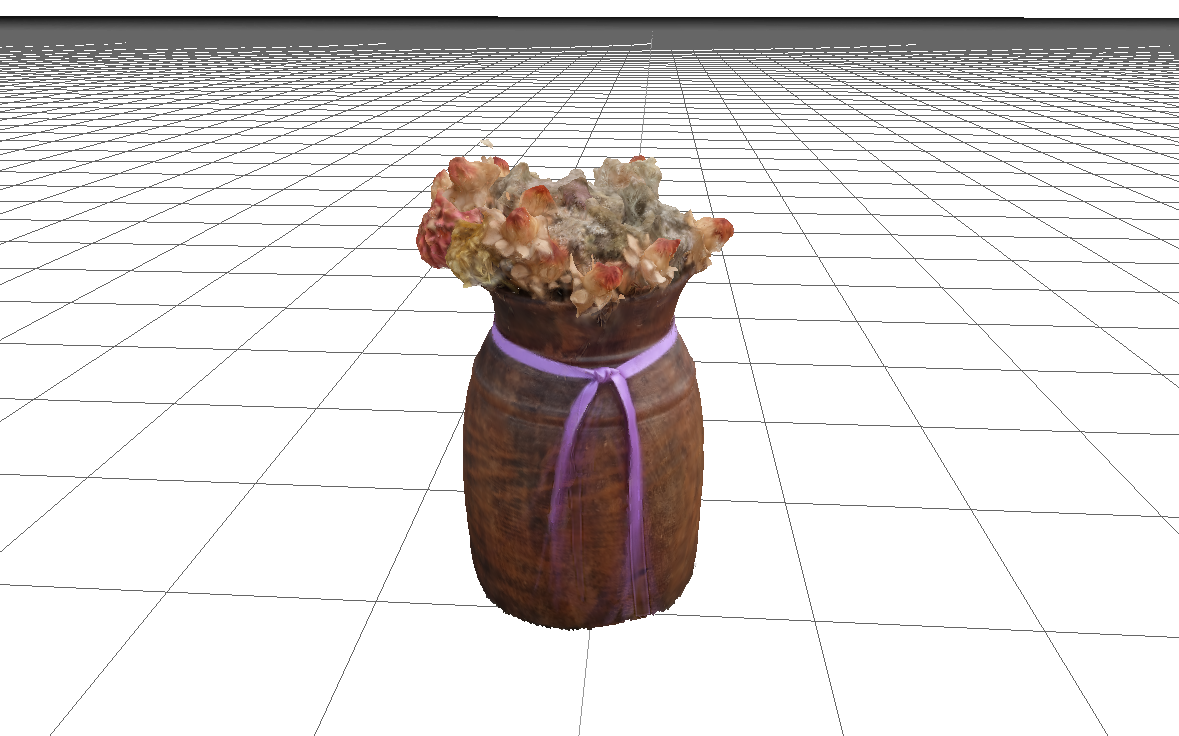
\includegraphics[width=\linewidth]{img/pianta.png}
    \caption{Oggetto ricostruito da Zephyr.}
  \end{subfigure}
  \captionsetup{justification=centering}
  \caption{Un vaso di fiori (40 foto); nonostante il basso livello di contrasto fra i fiori e lo sfondo zephyr ha ricreato l'oggetto egregiamente}
\end{figure}
Successivamente abbiamo utilizzato i tool per il mascheramento e la modifica degli oggetti messi a disposizione dal software Zephyr per capire come effettuare delle semplici modifiche senza dover ricorrere ad altri software.
Questi strumenti servono principalmente per rimuovere eventuali sfondi o punti d'appoggio dall'oggetto creato.
\begin{figure}[H]
  \centering
  \begin{subfigure}[b]{0.37\linewidth}
    \centering
    \includegraphics[width=\linewidth]{img/coltello1.JPG}
    \caption{Oggetto reale da ricostruire.}
  \end{subfigure}
  \begin{subfigure}[b]{0.4\linewidth}
    \centering
    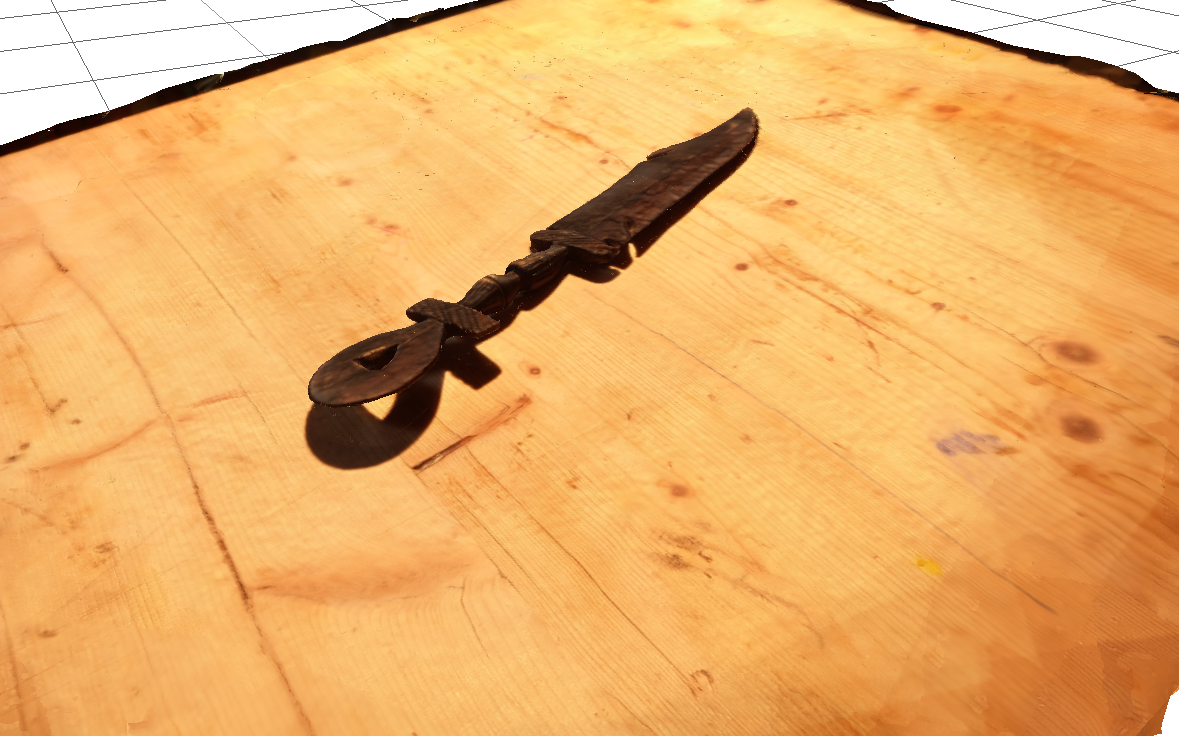
\includegraphics[width=\linewidth]{img/coltello.png}
    \caption{Oggetto ricostruito da Zephyr.}
  \end{subfigure}
  \captionsetup{justification=centering}
  \caption{Un coltello apribuste (50 foto), malgrado il lieve spessore la ricostruzione ha mantenuto fede ai dettagli}
\end{figure}

Ci siamo poi spinti oltre mettendo alla prova le capacit\`a di Zephyr di ricostruire elementi tridimensionali partendo da immagini con rumore gaussiano e successivamente elaborate con Matlab per ridurre il suddetto rumore.

Per iniziare abbiamo scattato le foto in una stanza buia con ISO pari a 25.600 per ricreare un rumore gaussiano senza per\`o ottenere il risultato sperato (probabilmente la macchina fotografica, Fujifilm X-T1, ha applicato in modo automatico un filtro antirumore) cos\`i abbiamo creato un filtro passa basso ideale con matlab:

\begin{equation}
H(u,v) = 
\begin{cases}
1,se D(u,v)\leq D_0
\\
0,se D(u,v)>D_0
\end{cases}
\end{equation}

\begin{equation}
D(u,v) = \sqrt{(u-M/2)^{2}) + (v-N/2)^{2})}   
\end{equation}
\newpage
 \noindent ottenendo il seguente risultato

\begin{figure}[H]
  \centering
  \begin{subfigure}[b]{0.45\linewidth}
    \centering
    \includegraphics[width=\linewidth]{img/pentola/original_noised.png}
    \caption{Immagine originale.}
  \end{subfigure}
  \begin{subfigure}[b]{0.45\linewidth}
    \centering
    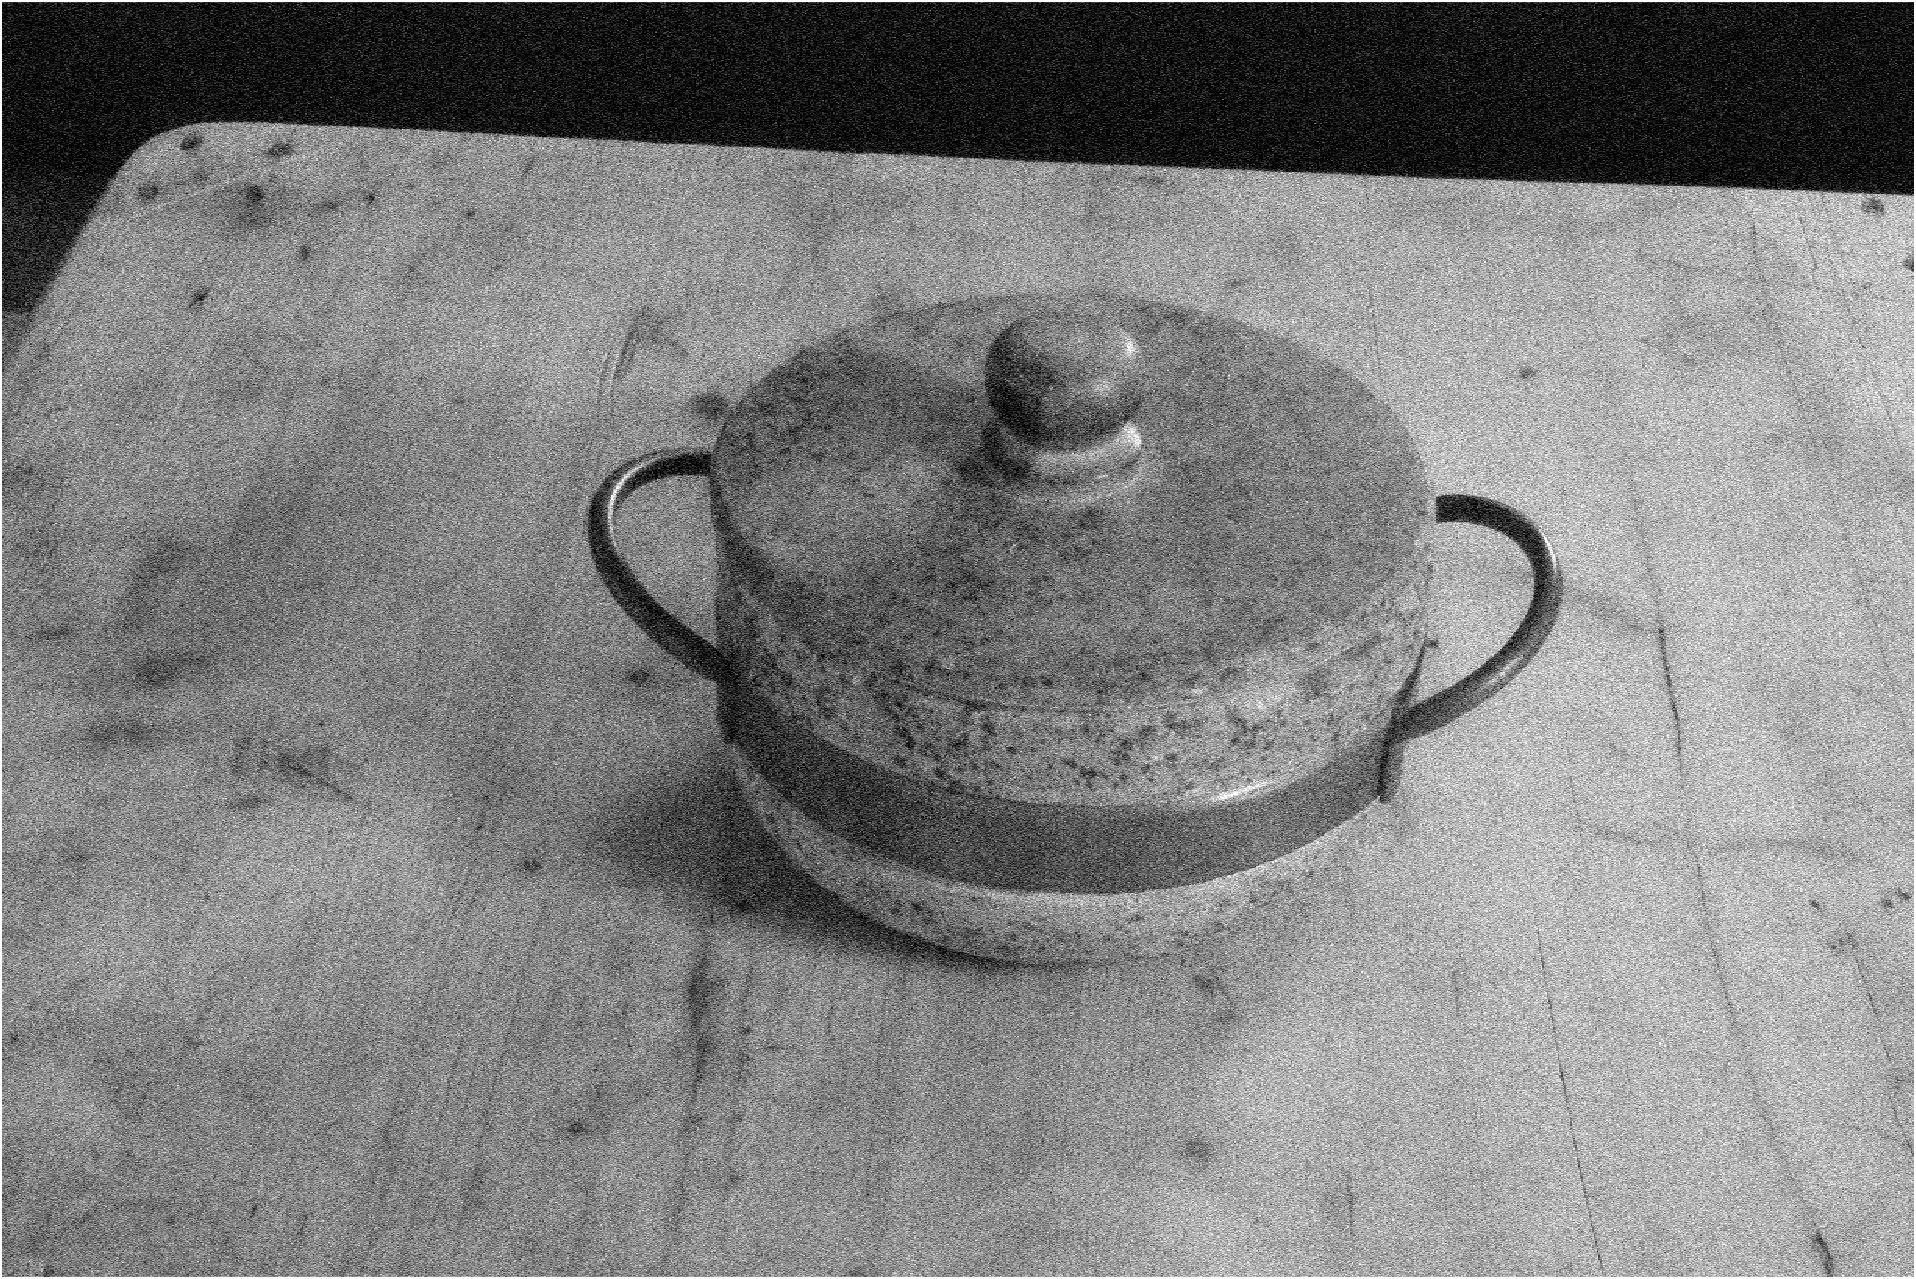
\includegraphics[width=\linewidth]{img/pentola/noised_image.png}
    \caption{Dopo aver applicato il rumore.}
  \end{subfigure}
\end{figure}

Togliendo il rumore generato grazie a matlab e deep learning si ottiene un risultato molto vicino all'originale. Per fare ci\`o è stato necessario convertire l'immagine da RGB a scala di grigi.

\textit{net = denoisingNetwork('DnCNN');\\denoisedI = denoiseImage(noisyI, net);\\figure\\imshow(denoisedI)\\title('Denoised Image')\\imwrite();}

\'E stato scelto questo procedimento perch\'e \`e quello che ha dato i risultati migliori.
%ORIGINALE -NOISED- DENOISED
\begin{figure}[H]
  \centering
  \begin{subfigure}[b]{0.4\linewidth}
    \centering
    \includegraphics[width=\linewidth]{img/pentola/original_noised.png}
    \caption{Immagine originale.}
  \end{subfigure}
  \begin{subfigure}[b]{0.4\linewidth}
    \centering
    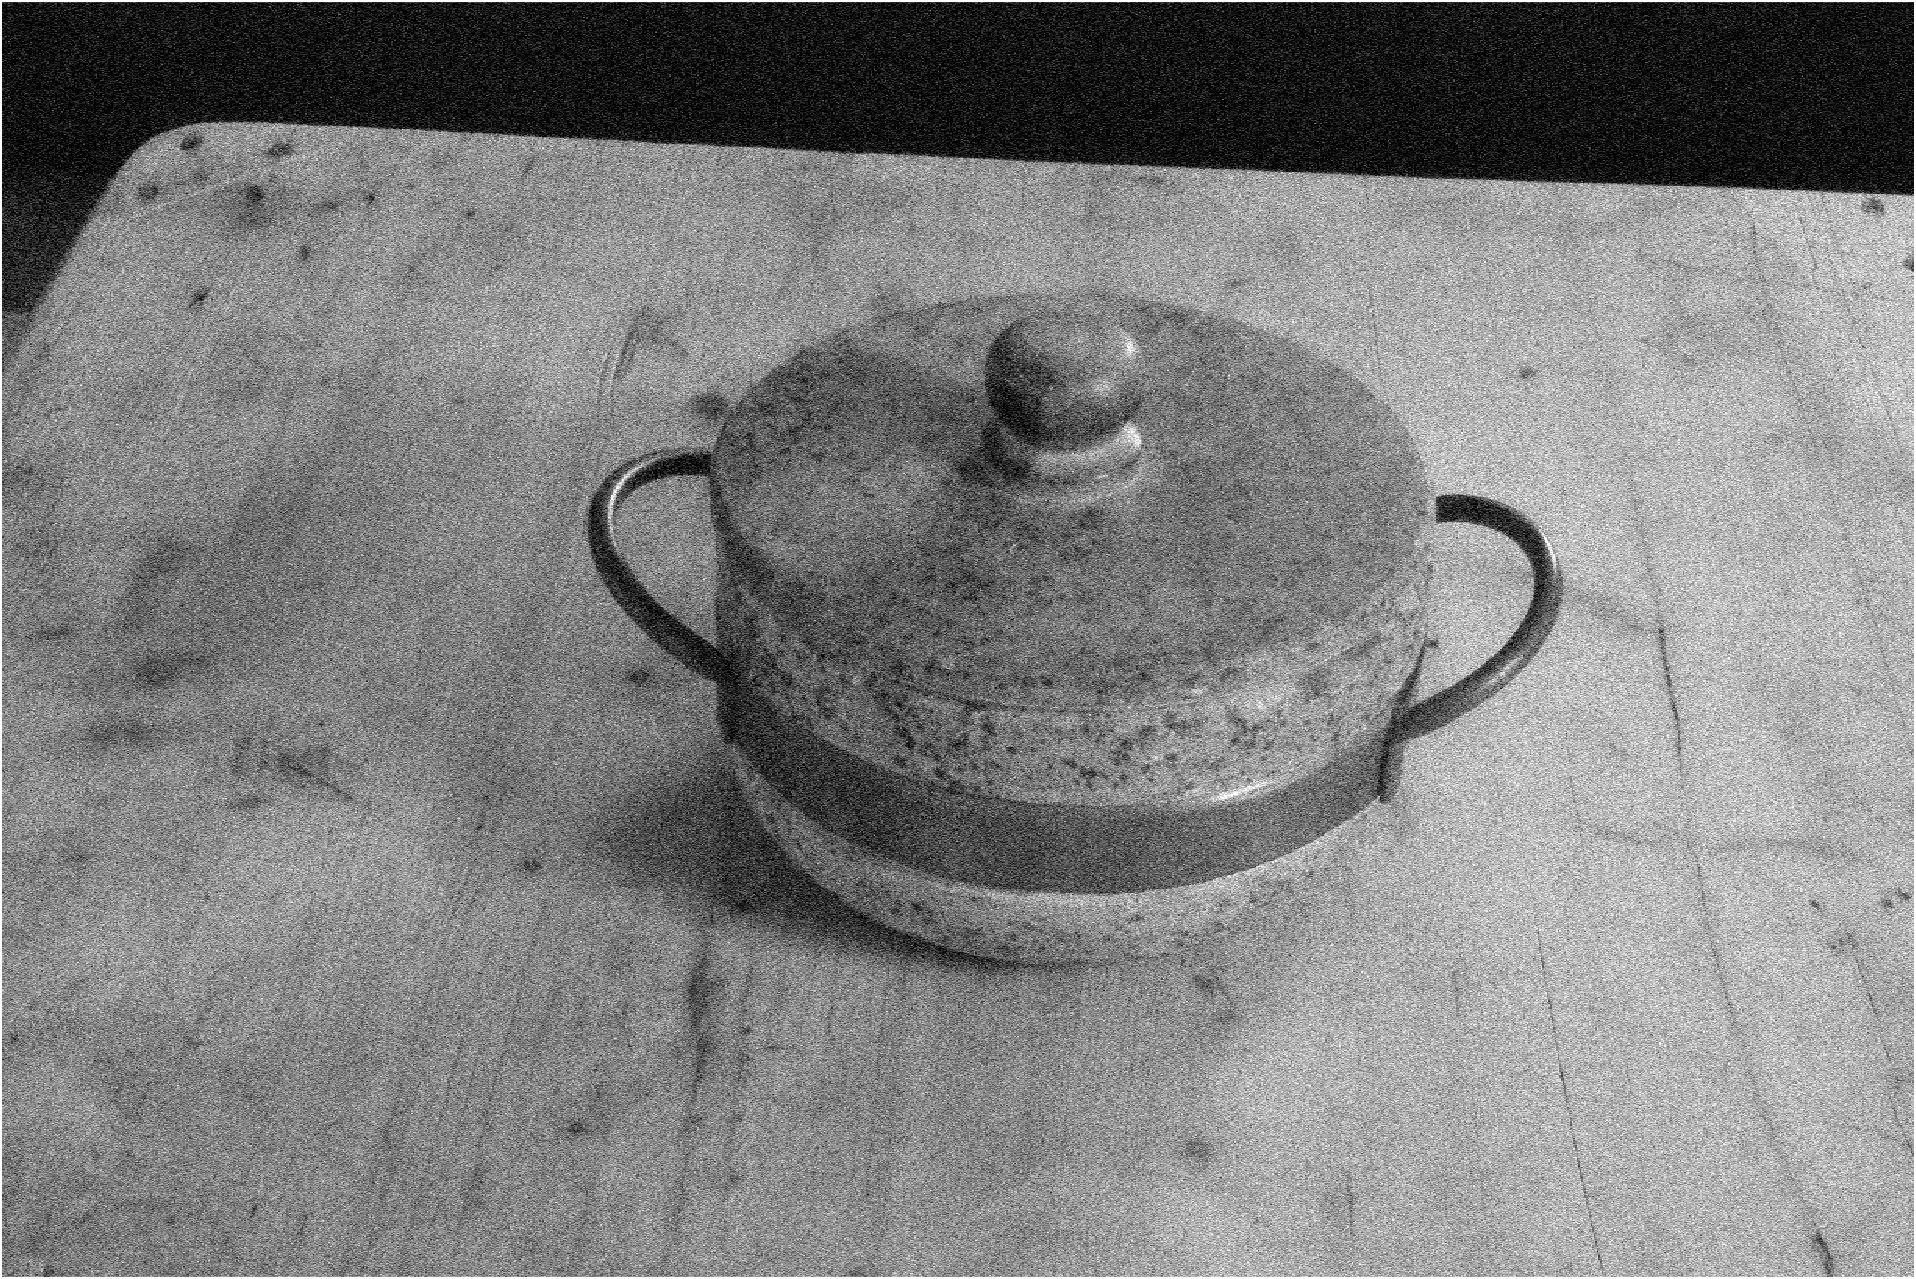
\includegraphics[width=\linewidth]{img/pentola/noised_image.png}
    \caption{Dopo aver applicato il rumore.}
  \end{subfigure}
  \begin{subfigure}[b]{0.6\linewidth}
    \centering
    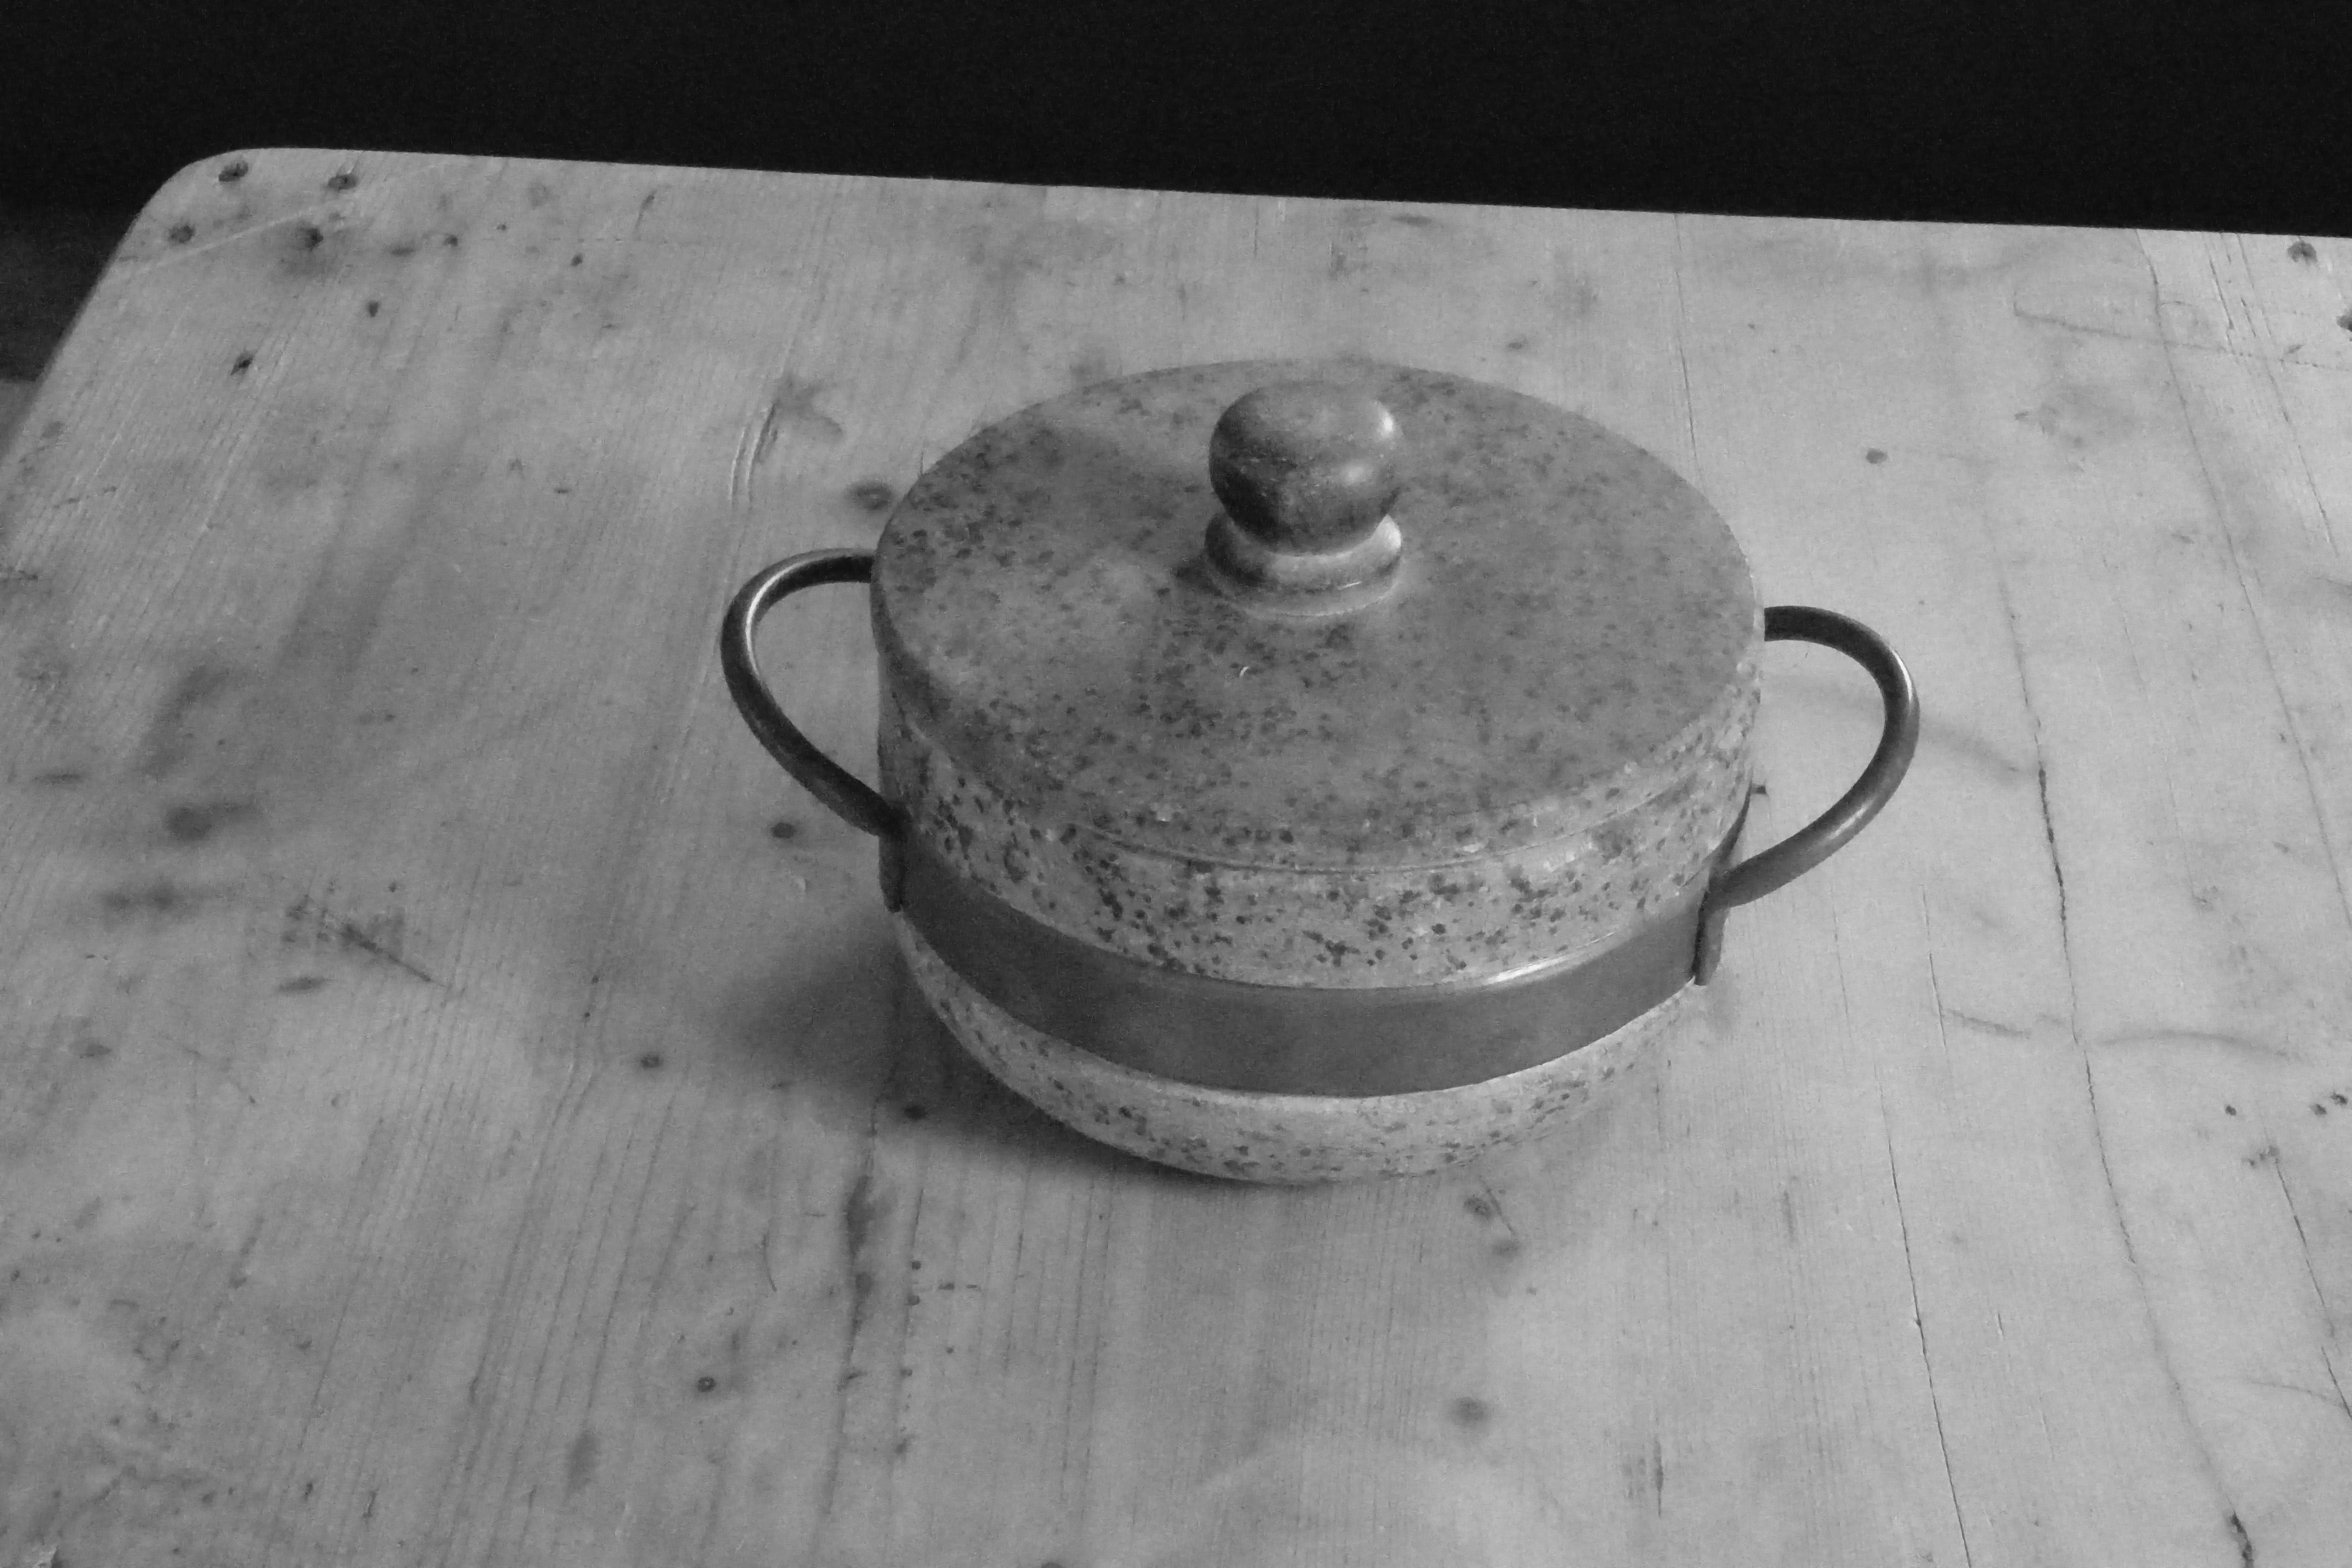
\includegraphics[width=\linewidth]{img/pentola/denoised_AI.jpg}
    \caption{Dopo aver tolto il rumore con MatLab}
  \end{subfigure}
\end{figure}

Abbiamo poi provato a sistemare un immagine fuori fuoco grazie all'algoritmo di convoluzione per rimuovere il blur dall'immagine:


\begin{equation}
f_1 * f_2 (t)  =  \int_{-\infty}^{\infty}{f_1(\tau)f_2 (t - \tau)d\tau}
\end{equation}

%BLURRED IMAGE - DEBLURRED IMAGE

\begin{figure}[H]
  \centering
  \begin{subfigure}[b]{0.35\linewidth}
    \centering
    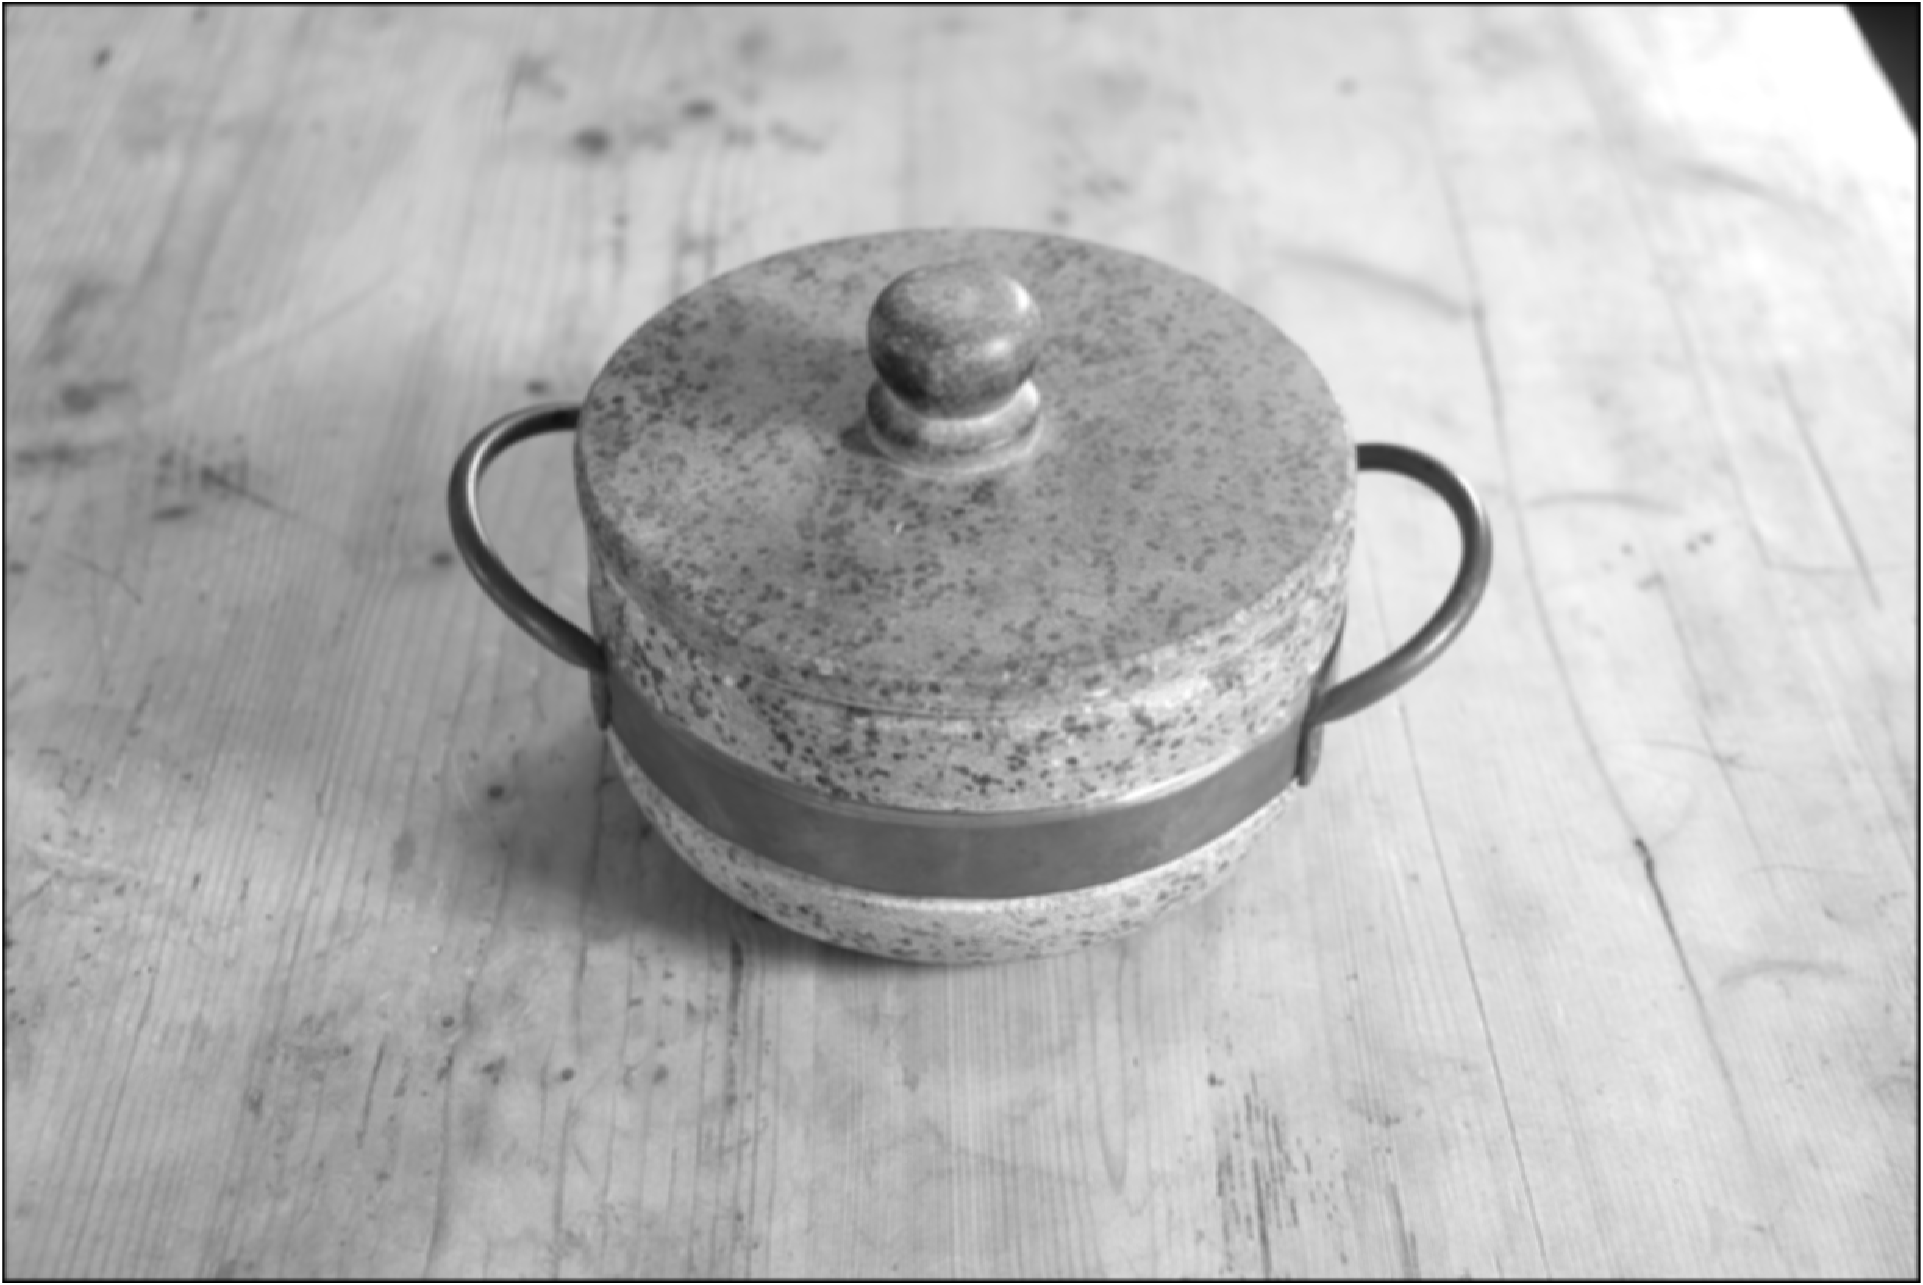
\includegraphics[width=\linewidth]{img/pentola/blurred_deconv.png}
    \caption{Immagine sfocata.}
  \end{subfigure}
  \begin{subfigure}[b]{0.35\linewidth}
    \centering
    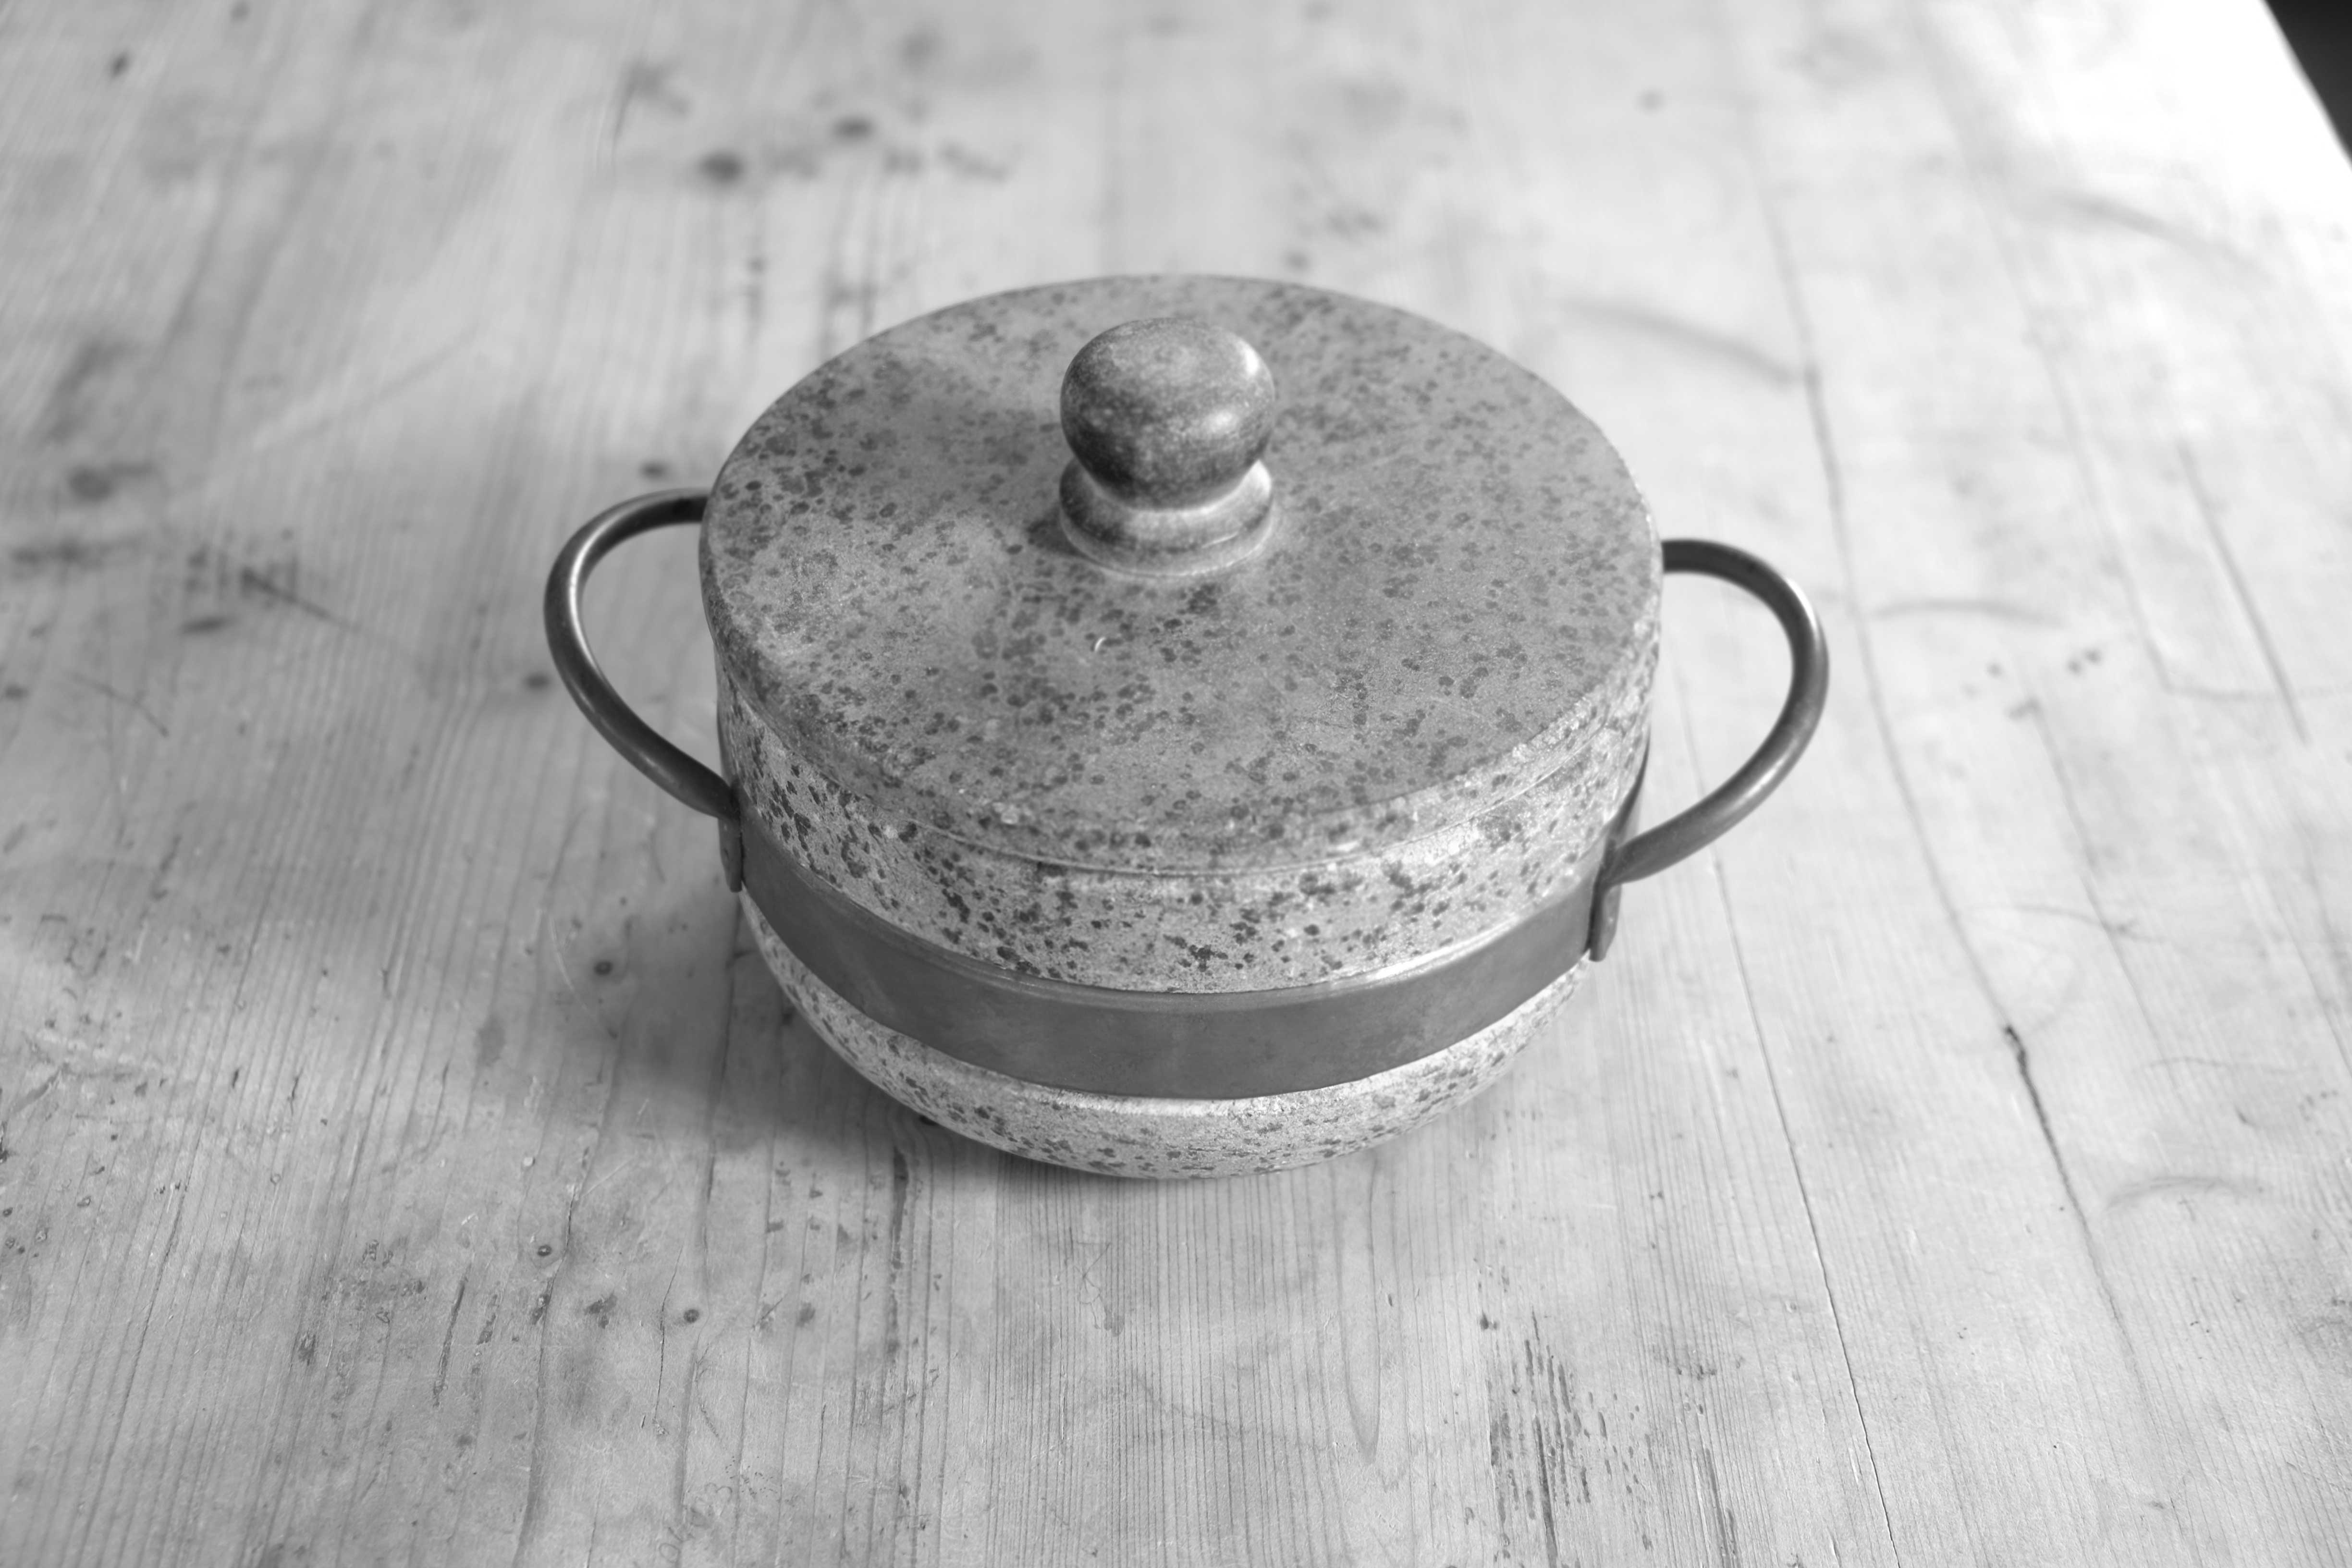
\includegraphics[width=\linewidth]{img/pentola/afuoco.jpg} %Sostituire
    \caption{Dopo l'algoritmo.}
  \end{subfigure}
\end{figure}

Infine abbiamo utilizzato le immagini restaurate per creare i modelli con zephyr ricavando dei risulati soddisfacenti. Nel caso della rimozione del rumore, trascurando la perdita del colore, l'oggetto ottenuto ha un qualit\`a quasi pari all'originale. Nel caso del blur la differenza sul pdf \`e meno percettibile ma si può comunque notare una riduzione della sfocatura.
%CONTINUA----------------------------------------------------------------

%OGGETTO ZEPHYR - OGGETTO GRAYSCALE DENOISED - GRAYSCALE DEBLURRED



\begin{figure}[H]
  \centering
  \begin{subfigure}[b]{0.45\linewidth}
    \centering
    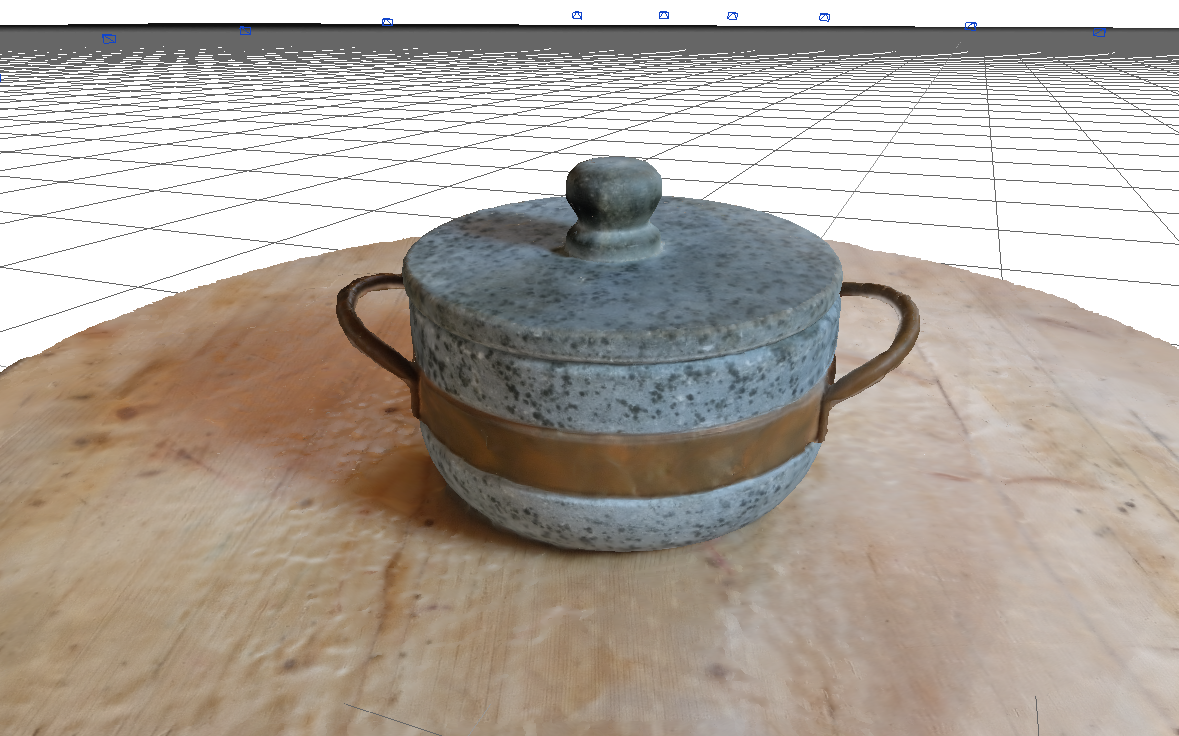
\includegraphics[width=\linewidth]{img/pentola/oggetto.png}
    \captionsetup{justification=centering}
    \caption{Oggetto reale ricostruito senza applicazione di filtri.} %sostituire
  \end{subfigure}
   \begin{subfigure}[b]{0.45\linewidth}
    \centering
    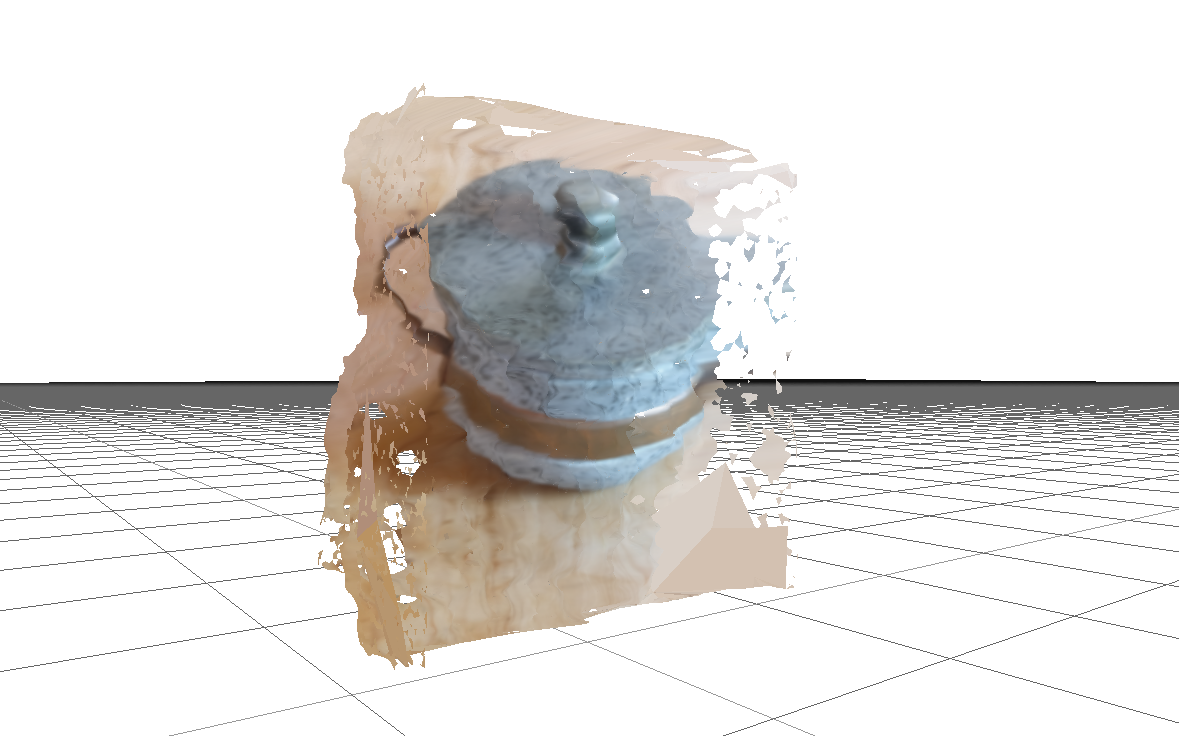
\includegraphics[width=\linewidth]{img/pentola/oggetto_blurred.png}
    \captionsetup{justification=centering}
    \caption{Oggetto ricostruito da immagini con rumore senza rinforzo.}
  \end{subfigure}
  \begin{subfigure}[b]{0.45\linewidth}
    \centering
    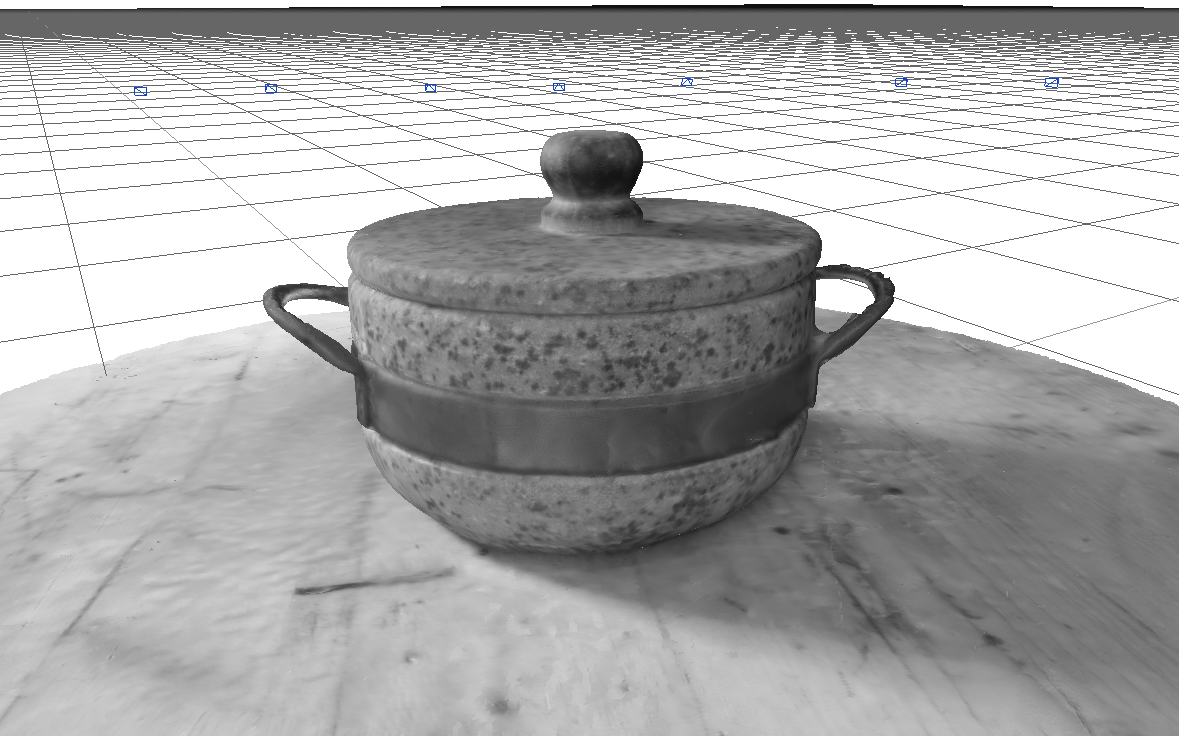
\includegraphics[width=\linewidth]{img/pentola/oggetto_grayscale.png} %sostituire
    \captionsetup{justification=centering}
    \caption{Oggetto ricostruito da immagini a cui \`e stato rimosso il rumore.}
  \end{subfigure}
  \begin{subfigure}[b]{0.45\linewidth}
    \centering
    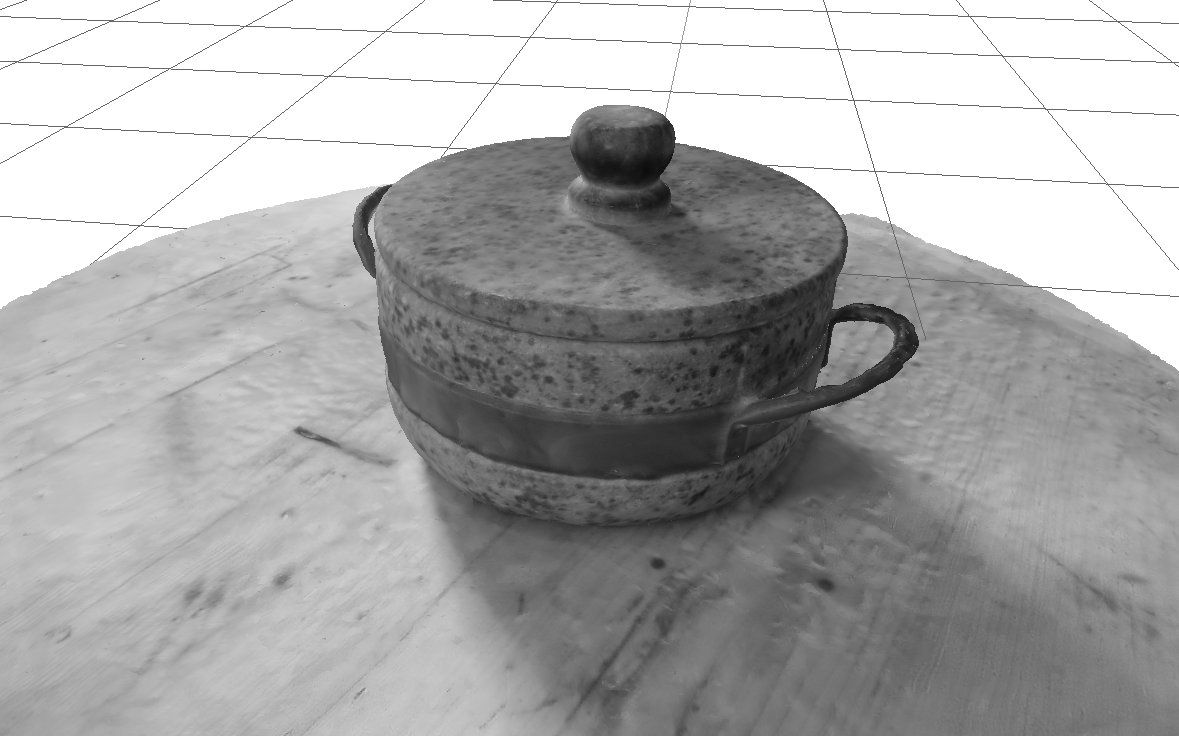
\includegraphics[width=\linewidth]{img/pentola/oggetto_deblurred.png}
    \captionsetup{justification=centering}
    \caption{Oggetto ricostruito da immagini a cui \`e stato rimosso il blur.}
  \end{subfigure}
  \captionsetup{justification=centering}
  \caption{Pentola (64 immagini), nel caso della ricostruzione con le immagini senza rinforzo zephyr non \`e riuscito ad elaborare tutte le immagine o parzialmente ed \`e stato ottenuto un risultato scadente, recuperato poi con il rinforzo delle immagini su matlab}
\end{figure}

\chapter{Ricostruzione e Fotogrammetria}
\section{Model Processing}
Come oggetto da ricostruire è stato scelto un oggetto reale di interesse storico ovvero una statua del Giardino Salvi di Vicenza e con il software Zephyr ne abbiamo riscostruito il modello 3D inserendolo successivamente all'interno del mondo di gioco.
Il processo per ricreare un oggetto adatto al funzionamento all'interno di un motore grafico  \`e composto da vari processi.
\subsection{Acquisizione delle immagini dell'oggetto da ricostruire}
Per acquisire il dataset ci siamo recati di pomeriggio in una giornata nuvolosa per evitare una eccessiva presenza di luce. Sono state utilizzate due fotocamere: una Fujifilm X-T1 e una Canon EOS 70D. Sono state scattate circa 700 foto da varie angolazioni per essere sicuri di acquisire la statua nella sua interezza.
\subsection{Elaborazione del dataset}
Bisogna assicurarsi che ogni foto all'interno del set abbia i requisiti per ricostruire un modello di buona qualit\`a; bisogna escludere quindi le immagini con esposizione troppo bassa o troppo alta, immagini mosse o sgranate perch\`e  anche una piccola percentuale di foto di bassa qualit\`a possono compromettere il risultato finale.
\newline
Se le immagini sono state catturate in formato RAW \`e necessario convertirle in un formato che sia adatto al programma di ricostruzione, per mantenere la miglior qualit\`a \`e consigliato convertirle nel formato TIFF, per questo si pu\`o utilizzare "Camera RAW" di Adobe oppure "DC RAW", un programma open-source creato da Dave Coffin.
\newline
Successivamente bisogna bilanciare i bianchi delle immagini acquisite mediante Adobe Photoshop.
\newline
Bisogna quindi convertire le immagini da 32 bit a 8 bit, questo per evitare problemi con la correzione di gamma all'interno del software di ricostruzione; in ogni caso la maggior parte dei software di ricostruzione converte in automatico le immagini a 8 bit, per cui non vi \`e perdita di informazioni.
\newline
Come ultimo passaggio abbiamo mascherato il nostro set di foto utilizzando 3DF Masquerade.

\begin{figure}[H]
    \centering
    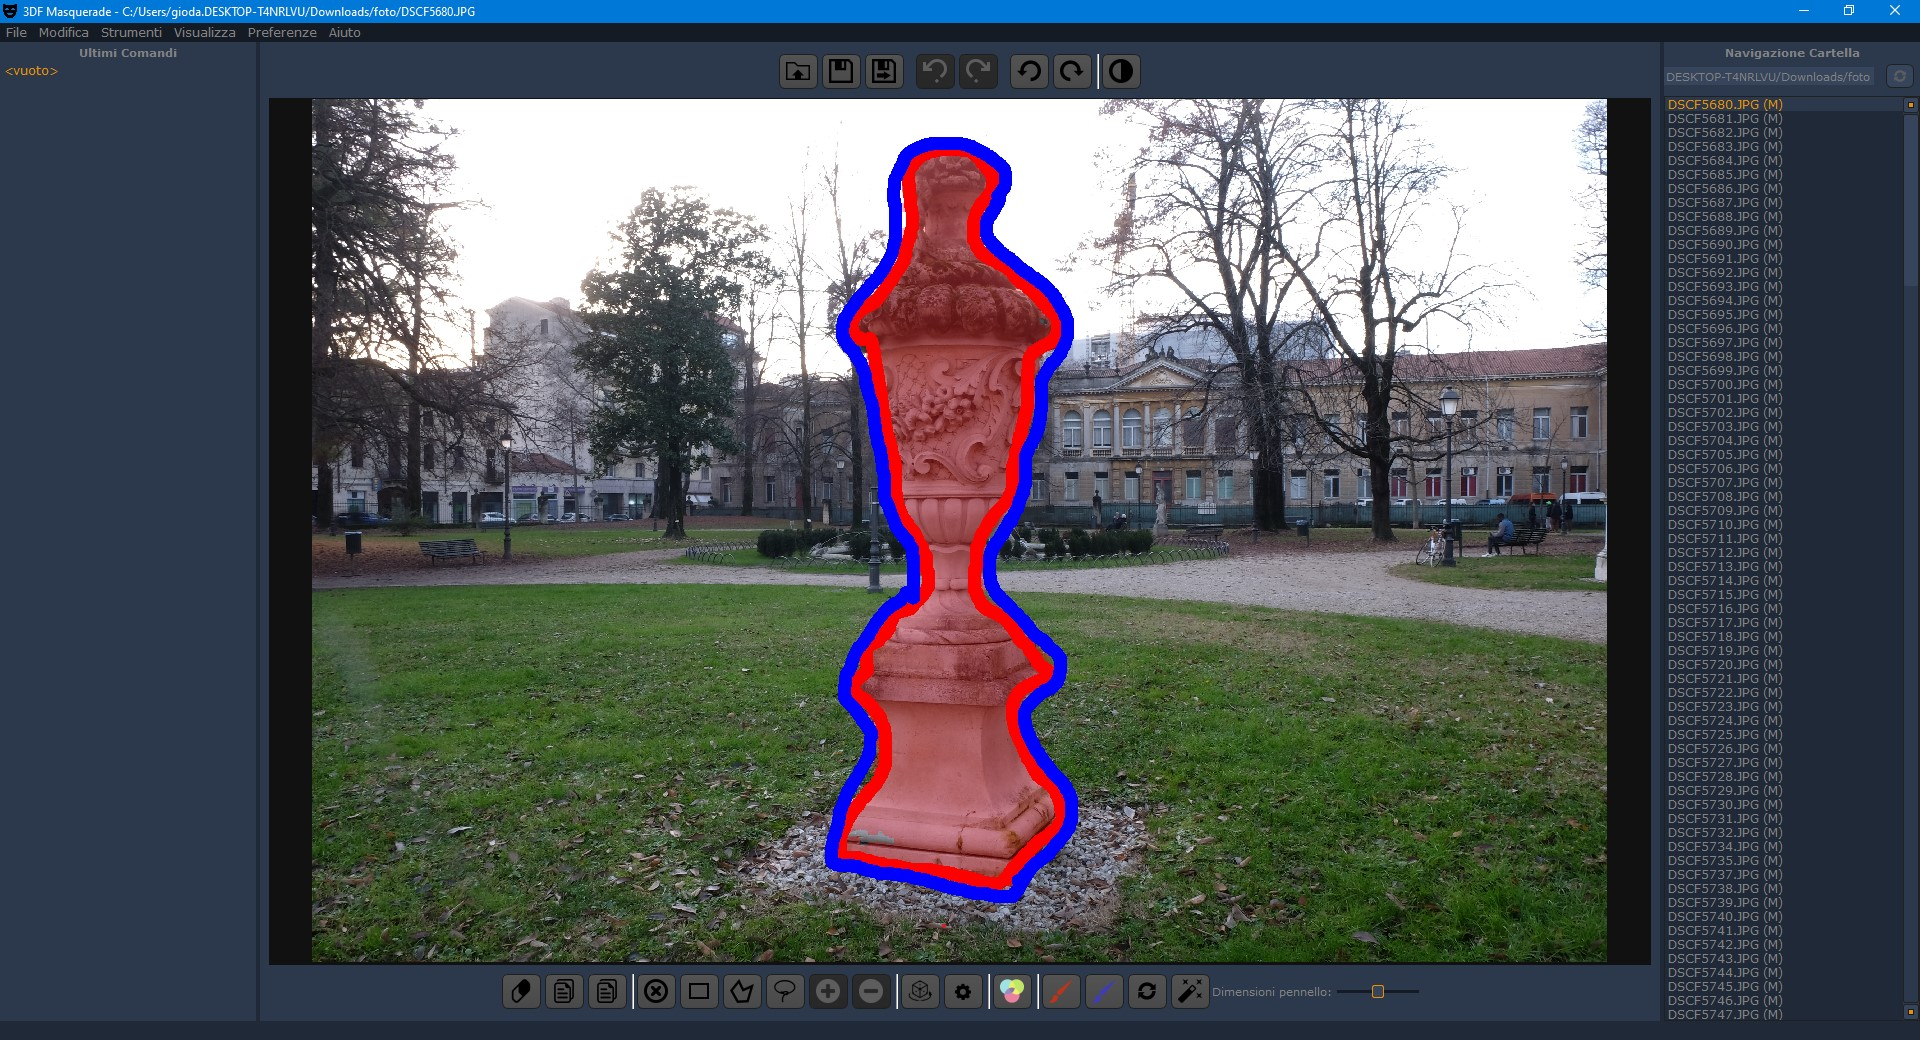
\includegraphics[width = \linewidth]{img/Mascherata.jpg}
    \caption{Una foto mascherata del nostro dataset all'interno del software 3DF Masquerade}
\end{figure}

\subsection{Ricostruzione dell'oggetto acquisito}
Per costruire l'oggetto principale della scena abbiamo utilizzato il software "Zephyr" di 3DFlow.
Aperto il programma abbiamo importato il nostro set di immagini (composto da 350 elementi), a questo punto abbiamo calcolato la nuvola di punti sparsa, la nuvola di punti densa, le mesh ad alta e a bassa risoluzione e infine la texture.
\begin{figure}[H]
    \centering
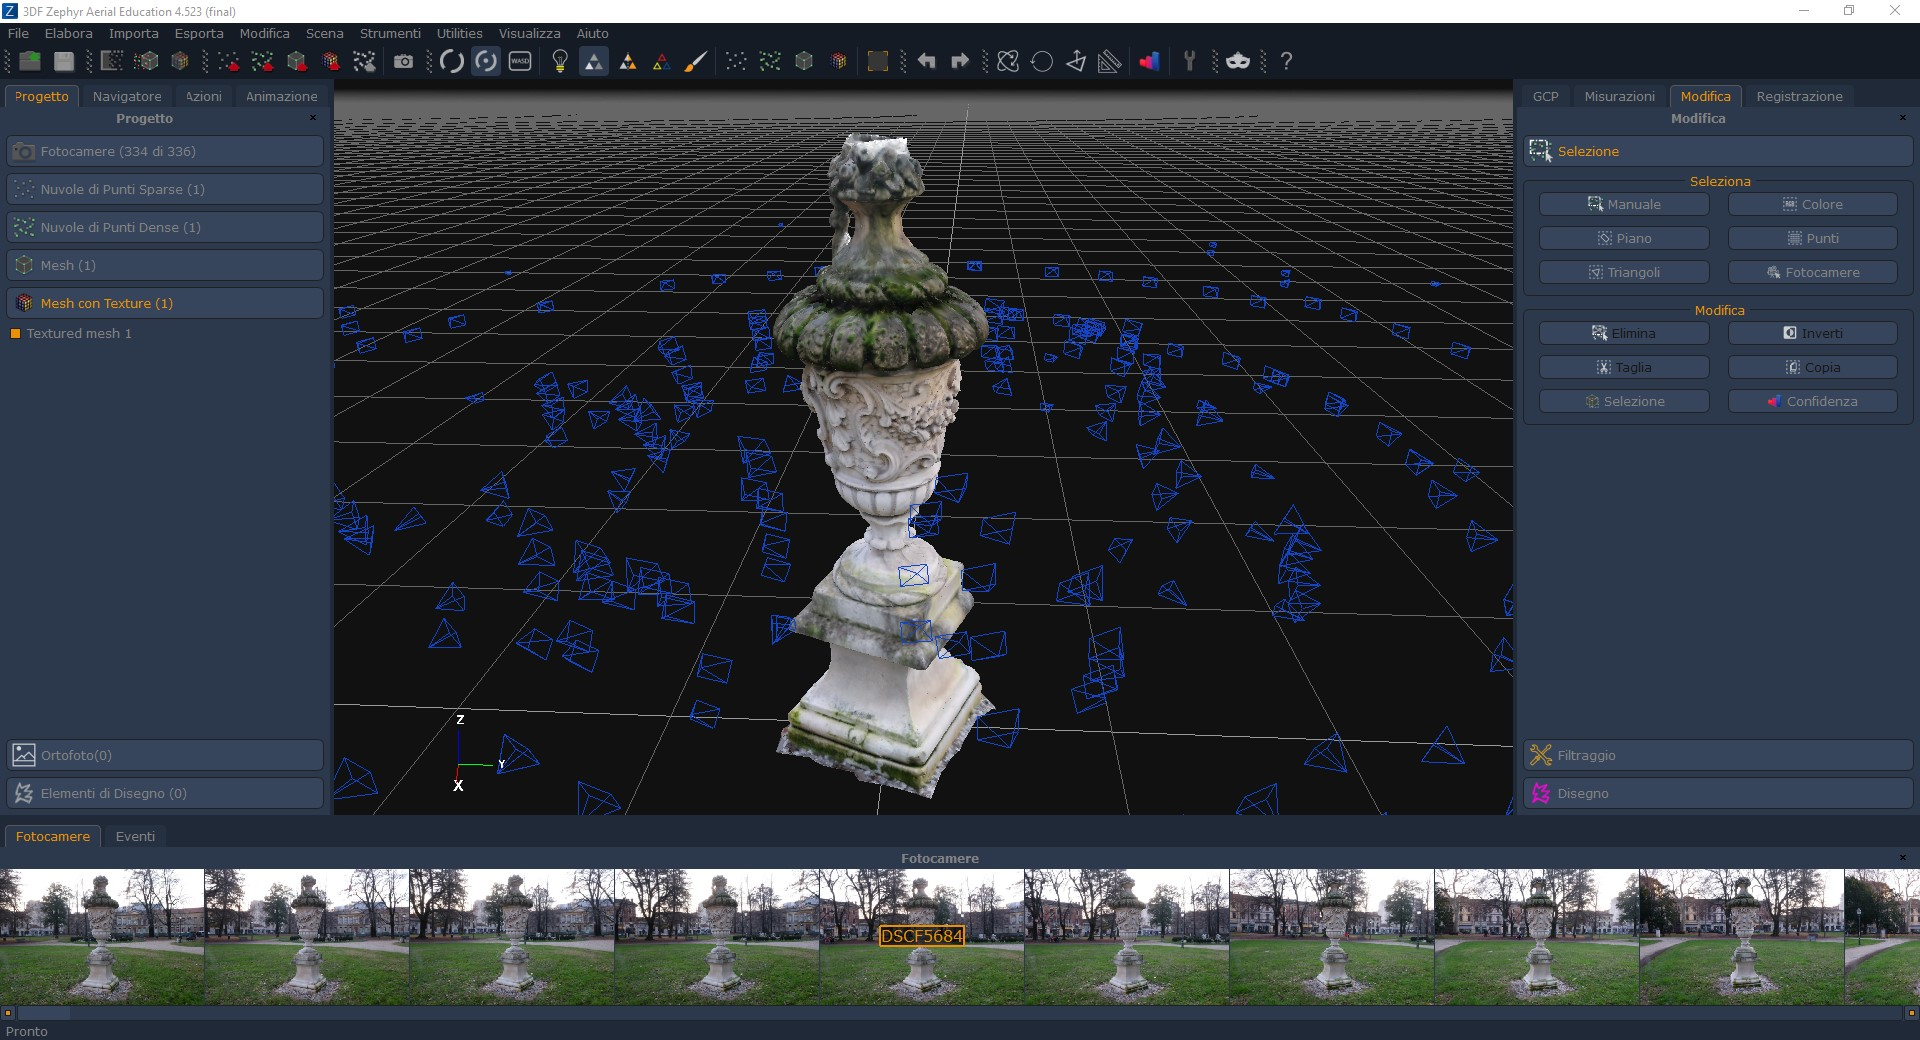
\includegraphics[width = \linewidth]{img/3DF_Zephyr_c.jpg}
    \caption{Mesh della statua ricostruita in 3DF Zephyr}
\end{figure}

\subsection{Baking delle normali}
Esportata la mesh ad alta risoluzione l'abbiamo importata nel programma "3DSMax" per calcolarne le normal map.
\begin{figure}[H]
    \centering
    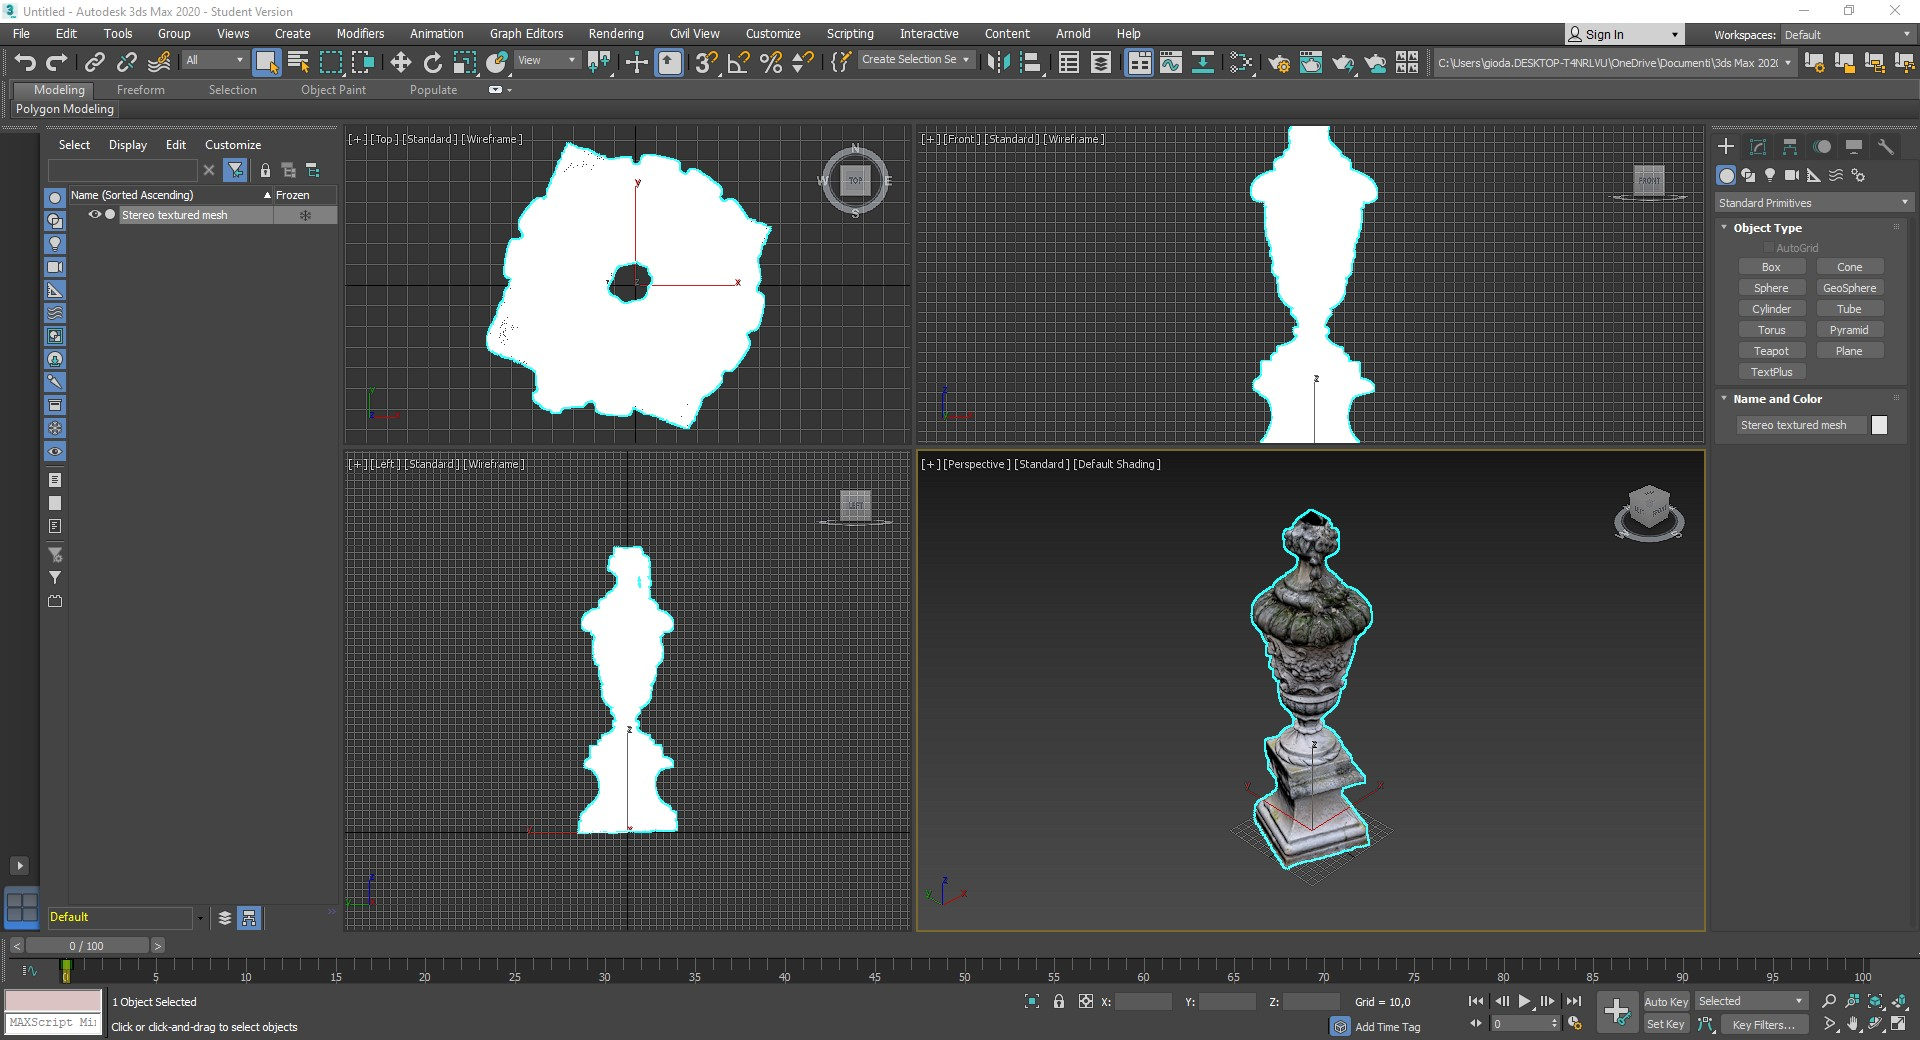
\includegraphics[width = \linewidth]{img/3DSMAX.jpg}
    \caption{Mesh ad alta risoluzione all'interno del software 3DSMAX}
\end{figure}

L'obiettivo \`e quello di effettuare il baking solo nelle alte frequenze della normal map per avere un materiale di dettagli elevati.

\subsection{Baking delle texture}
Per il processo di baking delle texture, ovvero il trasferimento dei dettagli dalla mesh ad alta risoluzione alla mesh a bassa risoluzione, abbiamo deciso di utilizzare il software "Knald" in quanto \`e risultato essere il pi\`u veloce e accurato nel nostro caso. Inoltre grazie al supporto del formato .ply ci ha concesso pi\`u flessibilit\`a per lavorare su Unity.
Abbiamo anche testato "Substance Designer" ma non abbiamo avuto gli stessi risultati soddisfacenti ottenuti con Knald.

\subsection{Pulizia della texture}
A questo punto abbiamo rimosso le luci e le ombre eccessive dalle texture. Per questo processo abbiamo utilizzato il software automatico di rimozione delle luci di Unity (Delightning tool). A volte il risultato di questo tool non è totalmente perfetto ed è consigliato utilizzare software aggiuntivo. Tuttavia nel nostro caso il risultato era più che buono poichè le texture non presentavano particolari problemi.

\subsection{Finalizzazione dell'oggetto ed esportazione dell'asset}
Dato che non avevamo bisogno delle texture ripetibili siamo passati alla finalizzazione e creazione dell'asset pronto per essere importato nella scena di Unity. Per fare ci\`o siamo nuovamente ricorsi al software 3DSMax.
\begin{figure}[H]
    \centering
    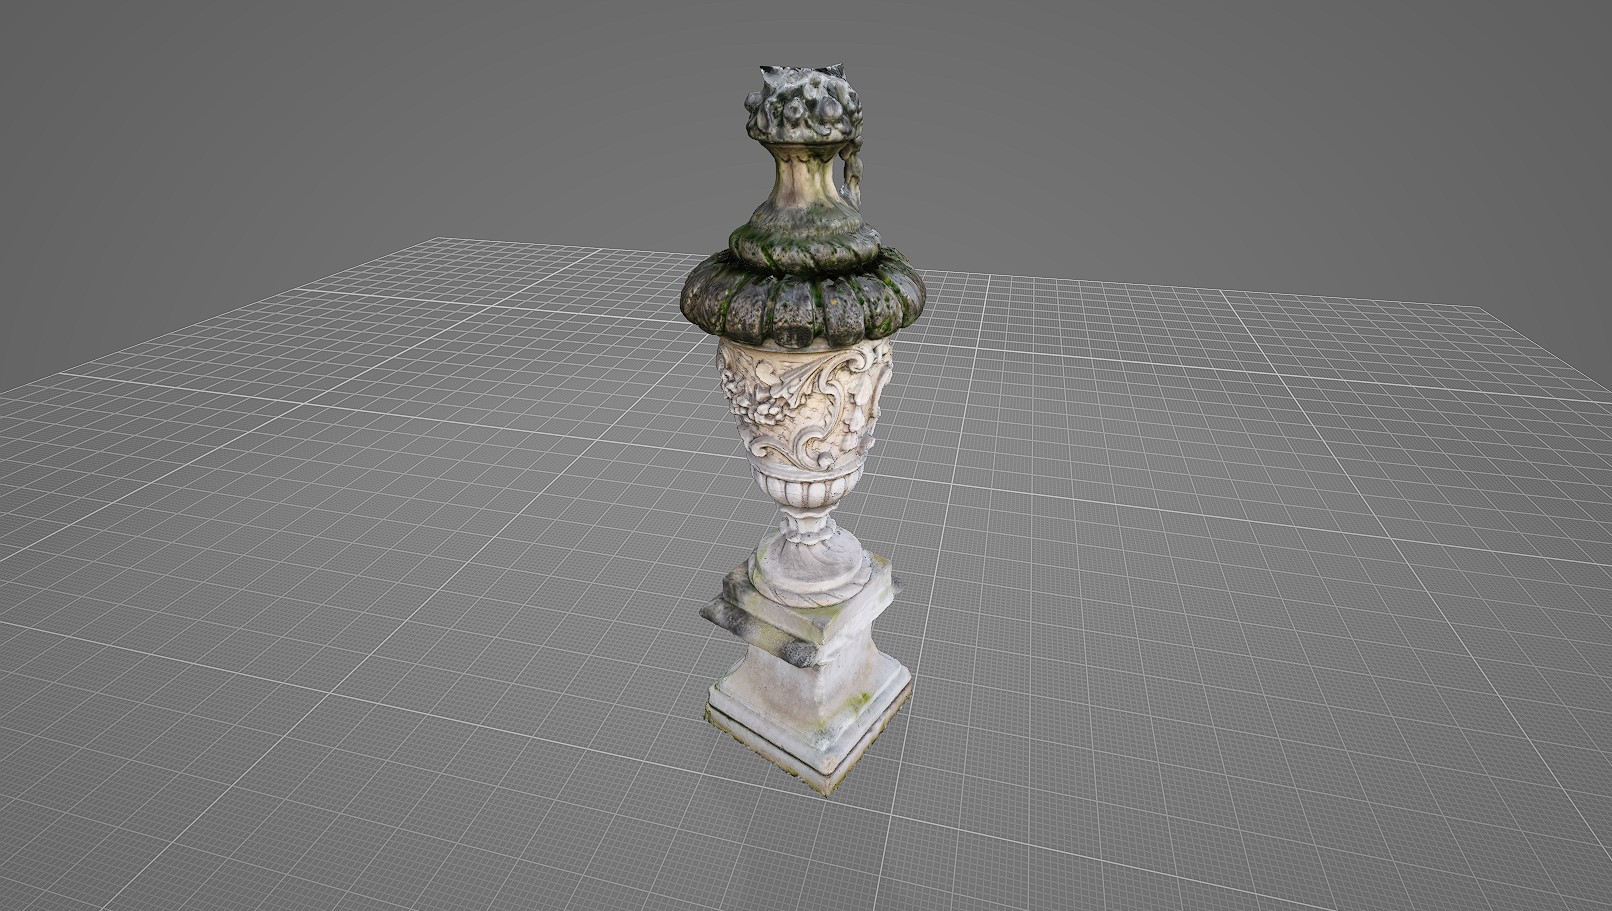
\includegraphics[width = 0.95\linewidth]{img/statua_fine.jpg}
    \caption{Risultato finale}
\end{figure}

\chapter{Creazione del gioco nel game engine Unity}
Per comporre la scena e gli oggetti creati con Zephyr ci siamo affidati al motore grafico pi\`u utilizzato al mondo: \textbf{Unity}

\begin{figure}[H]
    \centering
    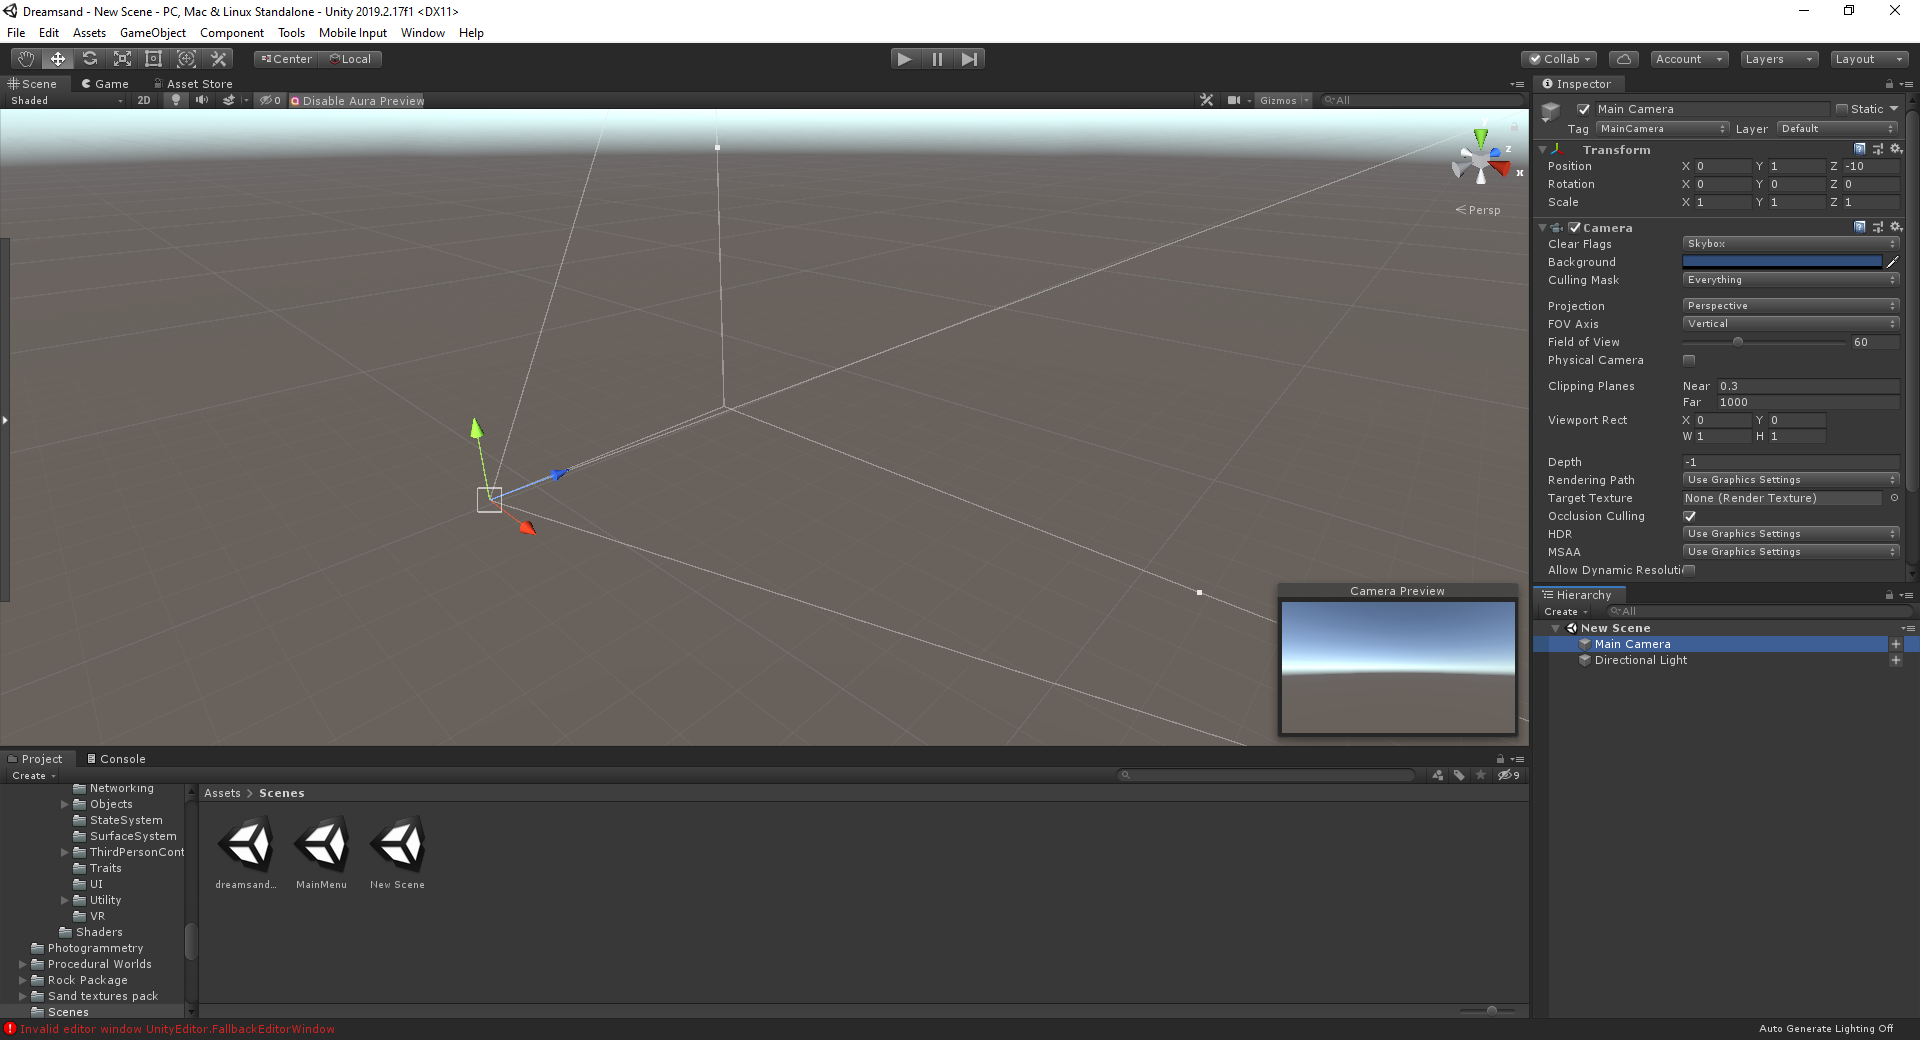
\includegraphics[width = \linewidth]{img/empty-scene.png}
    \caption{Una schermata dell'Editor di Unity}
\end{figure}

Per apprendere questo software ci siamo affidati alla documentazione ufficiale (\href{https://docs.unity3d.com/Manual/index.html}{Unity User Manual}) e alla sperimentazione sulle template gratuite create da Unity. (\href{https://assetstore.unity.com/packages/essentials/asset-packs/standard-assets-32351}{Standard Assets}).
Unity permette di creare giochi compatibili su diverse piattaforme dando allo sviluppatore tutti gli strumenti necessari per concentrarsi sulla creazione e non sull'ottimizzazione.

\section{Descrizione del gioco}
 Siamo partiti con l'intenzione di creare due livelli di gioco, uno più esplorativo in cui ci siamo concentrati maggiormente sui dettagli grafici dei singoli elementi che compongono la scena e l'altro più interattivo per dimostrare l'ottimizzazione dei modelli generati.
 
\subsection{Primo livello del gioco}
\subsubsection*{Ambientazione}
Il primo livello consiste in una zona desertica con al centro una piccola oasi protetta da delle piccole montagne, dalle quali sgorga una fonte d'acqua formando una piccola cascata. L'ambiente all'interno dell'oasi è caratterizzata da una folta vegetazione simile a quella pluviale, troviamo inoltre ponti sospesi che collegano varie zone sopraelevate.

%immagini dell'ambientazione dall'editor e all'interno del gioco
\begin{figure}[H]
  \centering
  \begin{subfigure}[b]{0.45\linewidth}
    \centering
    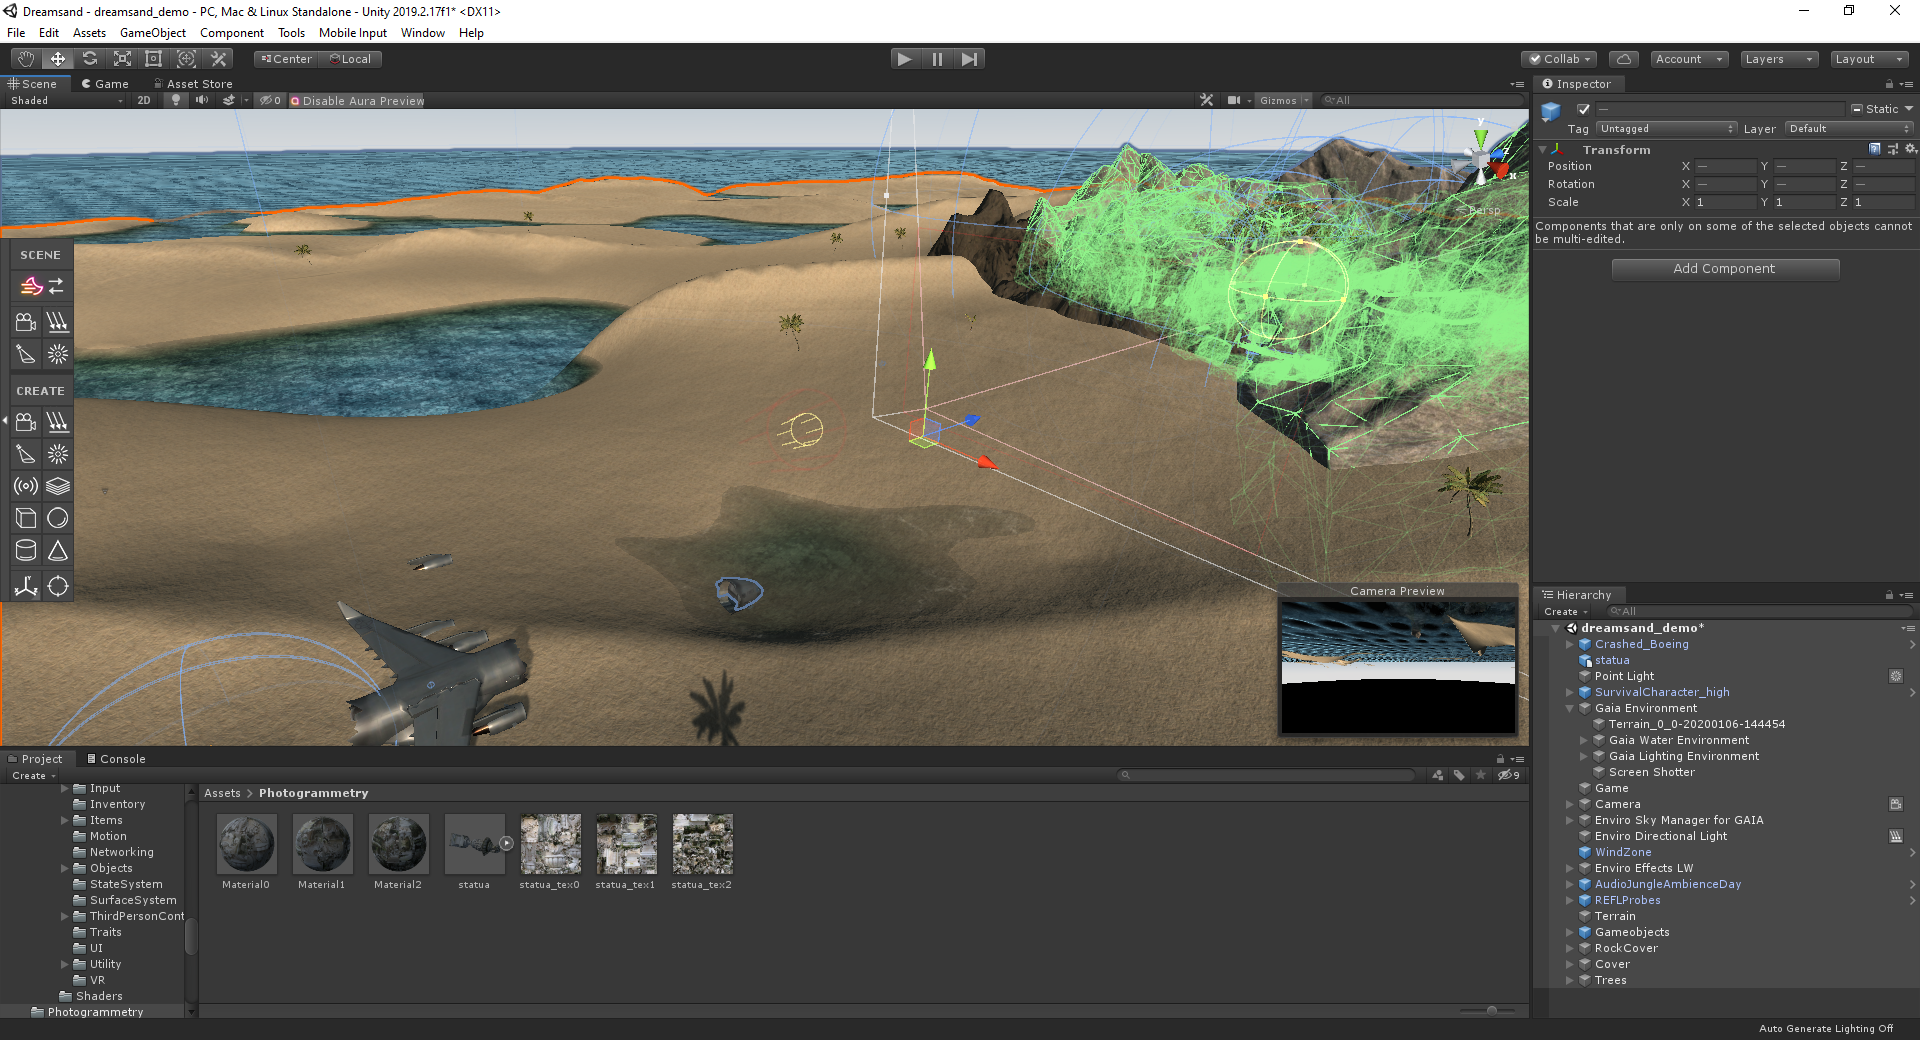
\includegraphics[width=\linewidth]{img/dreamsand-scene.png}
    \captionsetup{justification=centering}
    \caption{Area desertica vista dall'editor di Unity.}
  \end{subfigure}
   \begin{subfigure}[b]{0.45\linewidth}
    \centering
    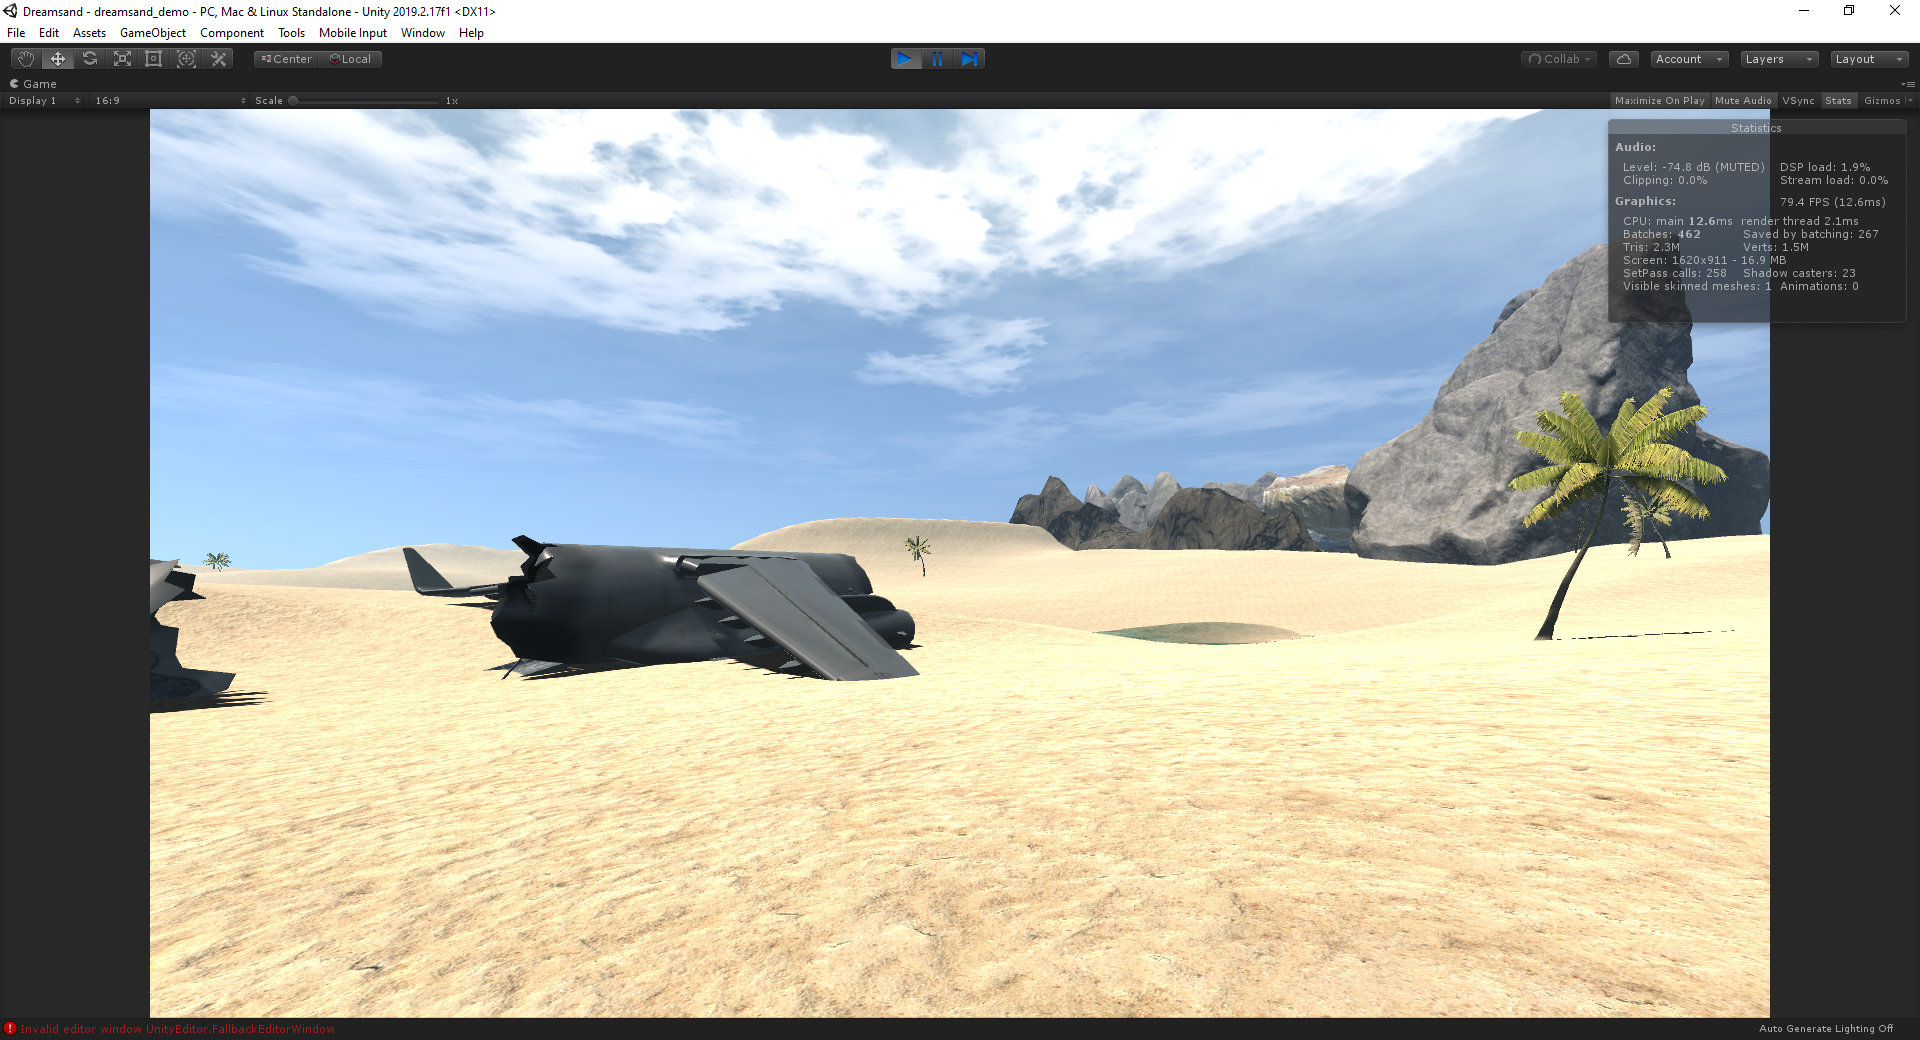
\includegraphics[width=\linewidth]{img/dreamsand-ingame.png}
    \captionsetup{justification=centering}
    \caption{Area desertica vista all'interno del gioco}
  \end{subfigure}
  \begin{subfigure}[b]{0.45\linewidth}
    \centering
    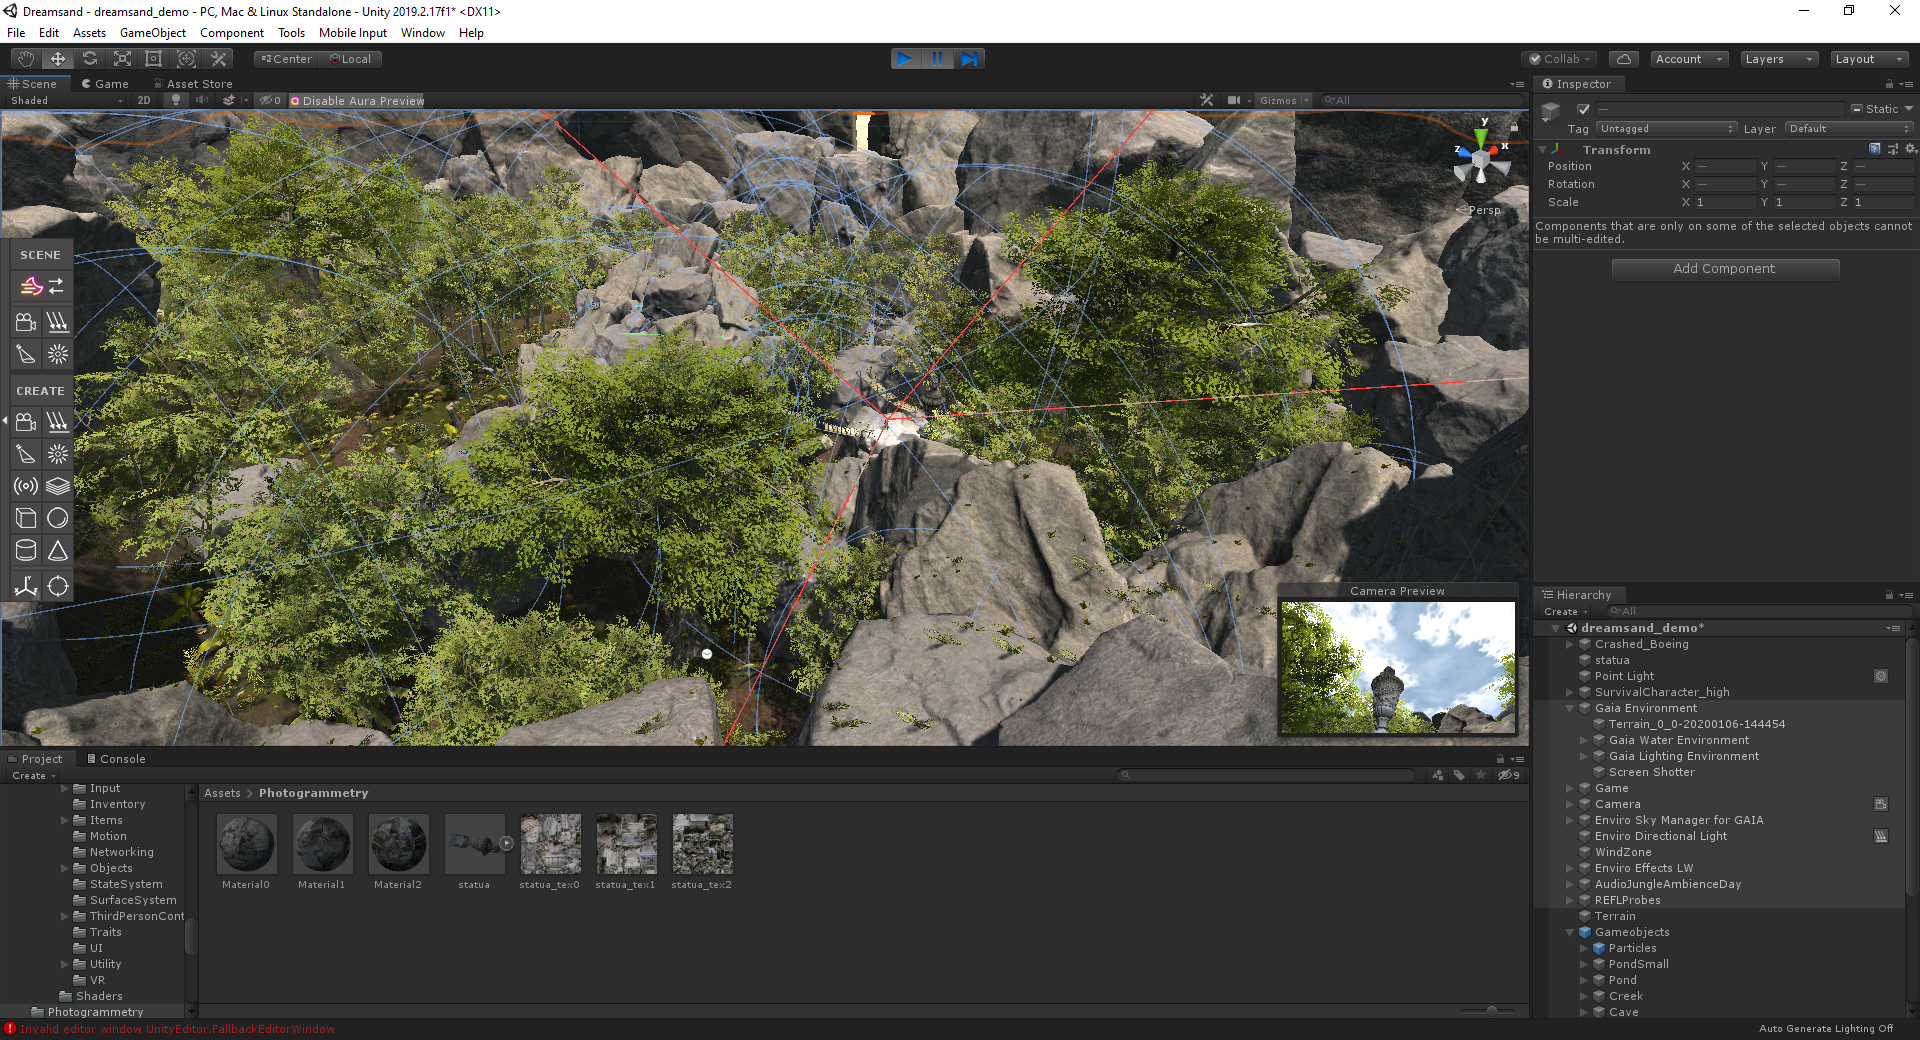
\includegraphics[width=\linewidth]{img/dreamsand-oasis-scene.png} %sostituire
    \captionsetup{justification=centering}
    \caption{L'oasi vista dall'editor di Unity.}
  \end{subfigure}
  \begin{subfigure}[b]{0.45\linewidth}
    \centering
    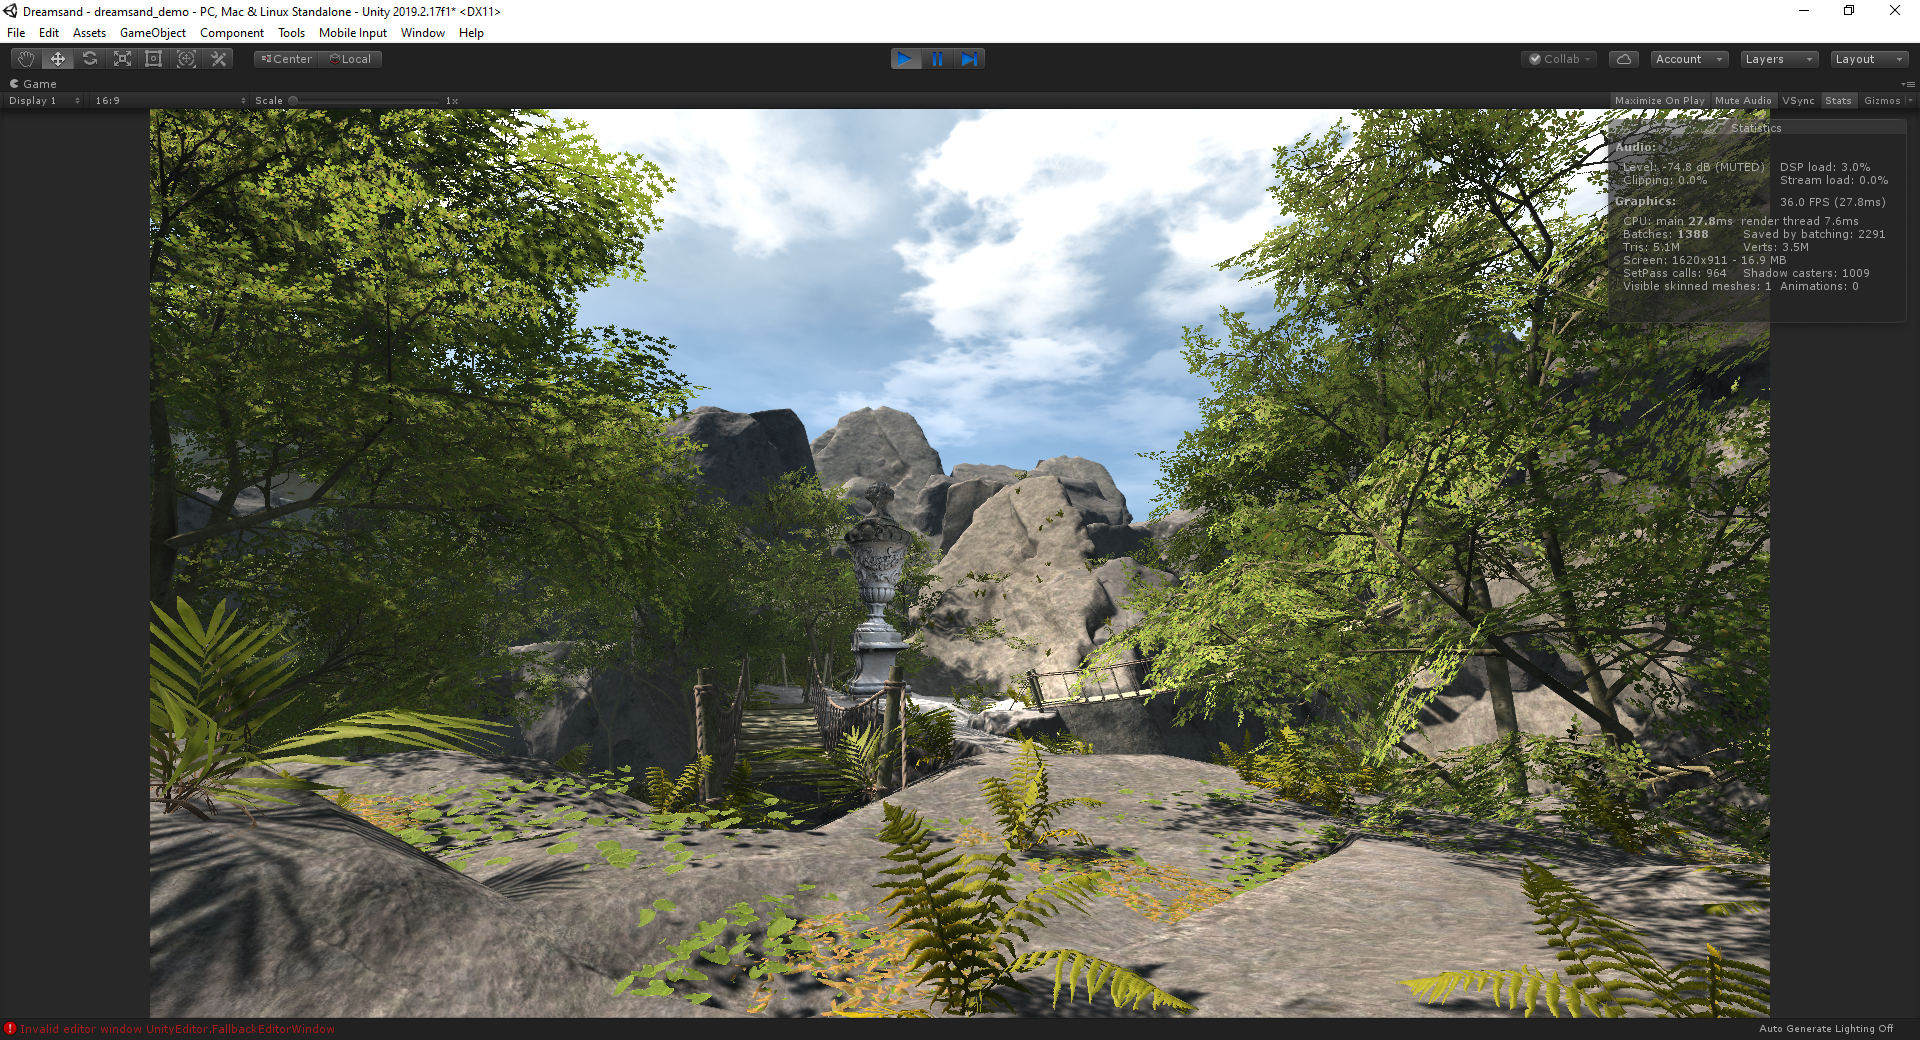
\includegraphics[width=\linewidth]{img/dreamsand-ingame-statue.png}
    \captionsetup{justification=centering}
    \caption{L'oasi vista all'interno del gioco}
  \end{subfigure}
\end{figure}

\subsubsection*{Gameplay}
L'obiettivo del primo livello è quello di esplorare l'ambiente di gioco cercando di trovare uno dei nostri oggetti ricostruiti tramite la fotogrammetria, in questo caso la statua ricostruita nella sezione precedente.

%Inserire immagine della statua nel gioco
\begin{figure}[H]
    \centering
    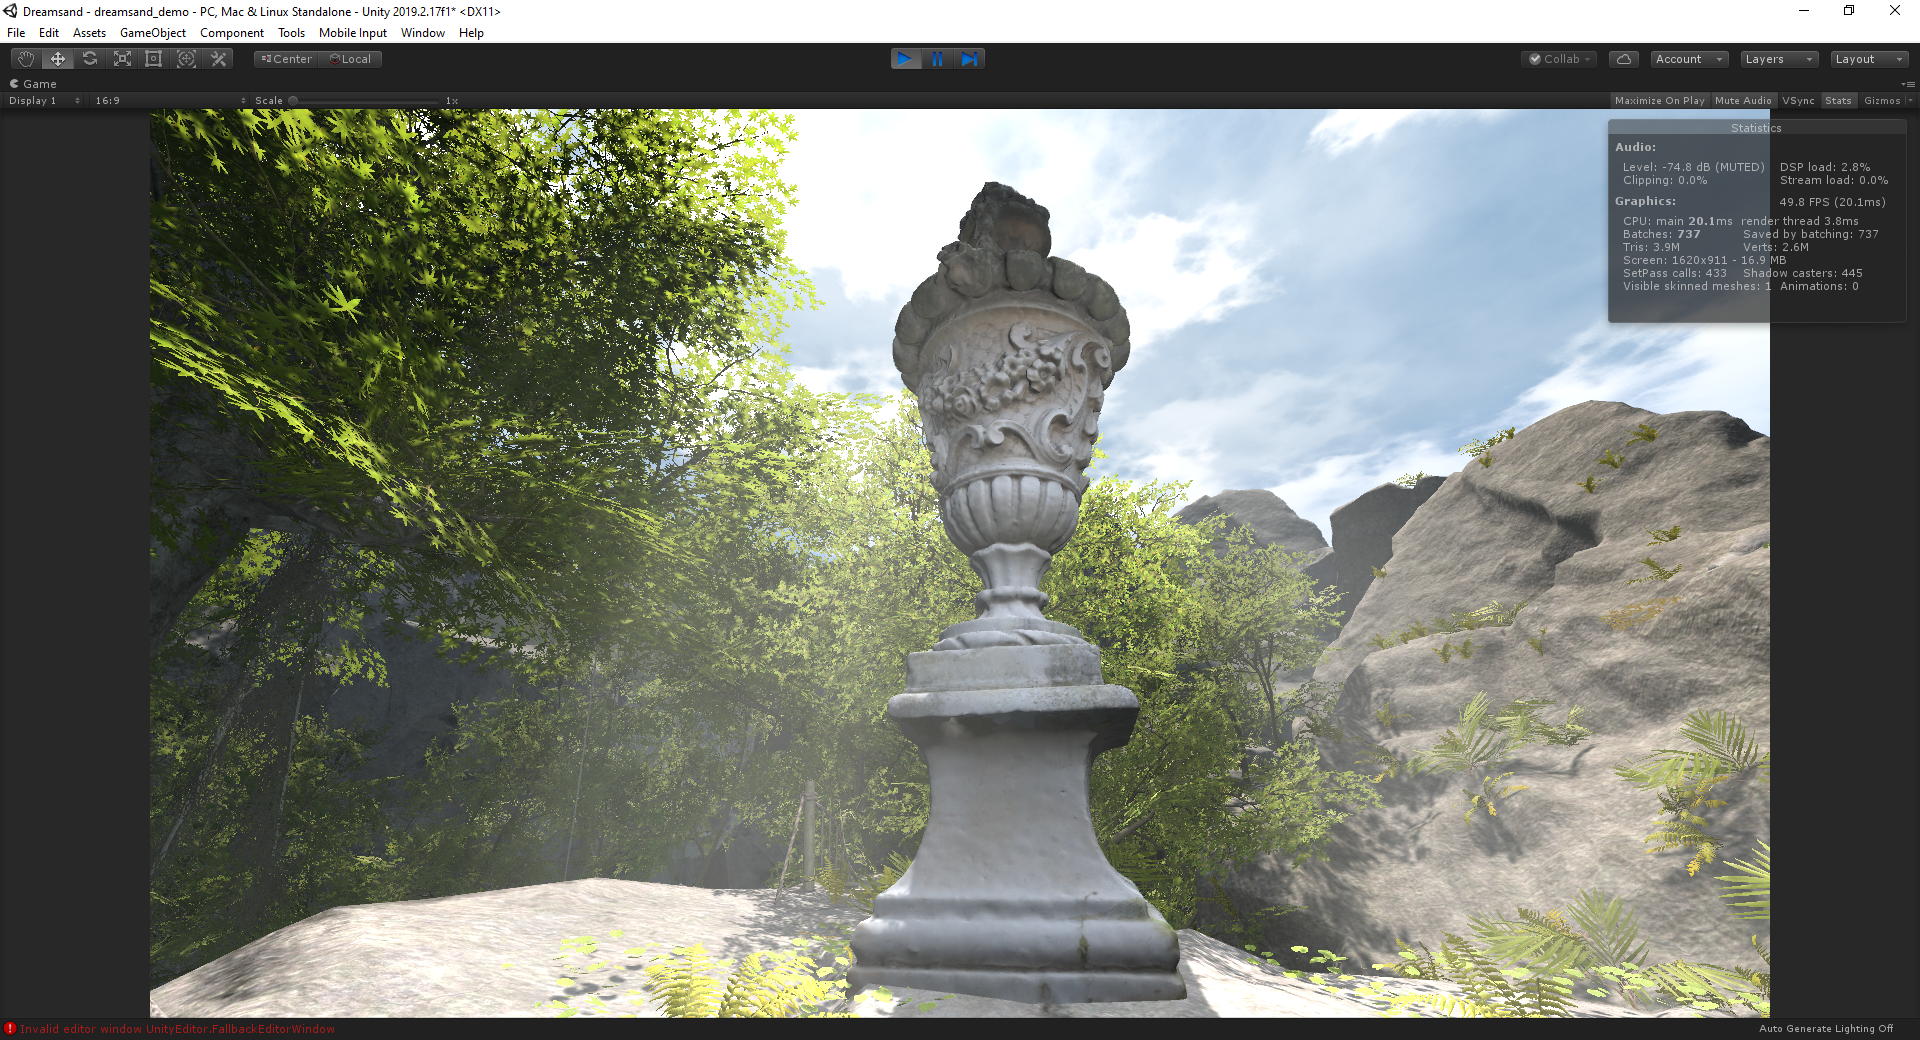
\includegraphics[width = \linewidth]{img/dreamsand-ingame-statue-close.png}
    \caption{L'asset della statua all'interno del gioco}
\end{figure}

Nel corso dell'esplorazione il giocatore dovr\`a essere cauto, in quanto una caduta da una determinata altezza comporter\`a la morte del protagonista.

\subsubsection*{Tecniche utilizzate}
\begin{itemize}
    \item Per ridurre il carico di lavoro della gpu abbiamo utilizzato un algoritmo LOD (level of detail). Il LOD riduce la complessità della rappresentazione del modello 3D in base alla distanza dell'osservatore oppure basate su altre metriche come l'importanza di un oggetto oppure la velocit\`a relativa al punto di vista.
    \item Per i collider abbiamo preferito utilizzare i \textit{mesh collider} ai \textit{box collider} ove possibile. I mesh collider prendono la mesh dell'asset e costruiscono i collider basandosi sulla suddetta mesh. 
    La mesh è una collezione di vertici (vertex), bordi(edge) e facce(face) che descrivono la forma di un oggetto 3D. Un vertice \`e un singolo punto, un bordo(edge) \`e un segmento che connette due vertici e infine una faccia è una superficie piana racchiusa tra bordi(edges).
    \item Per definire la forma dei nostri oggetti all'interno dello spazio 3D abbiamo utilizzato la tecnica del Mesh renderer. Questa tecnica prende la geometria del filtro delle mesh e ne reindirizza la posizione definita dalla componente di trasformazione del game object.
\end{itemize}

\subsection{Secondo livello del gioco}
\subsubsection*{Ambientazione}
Il protagonista si ritrover\`a su di una scacchiera con relativi pezzi a grandezza d'uomo. L'ambiente circostante è assente se non per una skybox per dargli una parvenza surreale.

%immagini dell'ambientazione dall'editor e all'interno del gioco
\begin{figure}[H]
  \centering
  \begin{subfigure}[b]{0.45\linewidth}
    \centering
    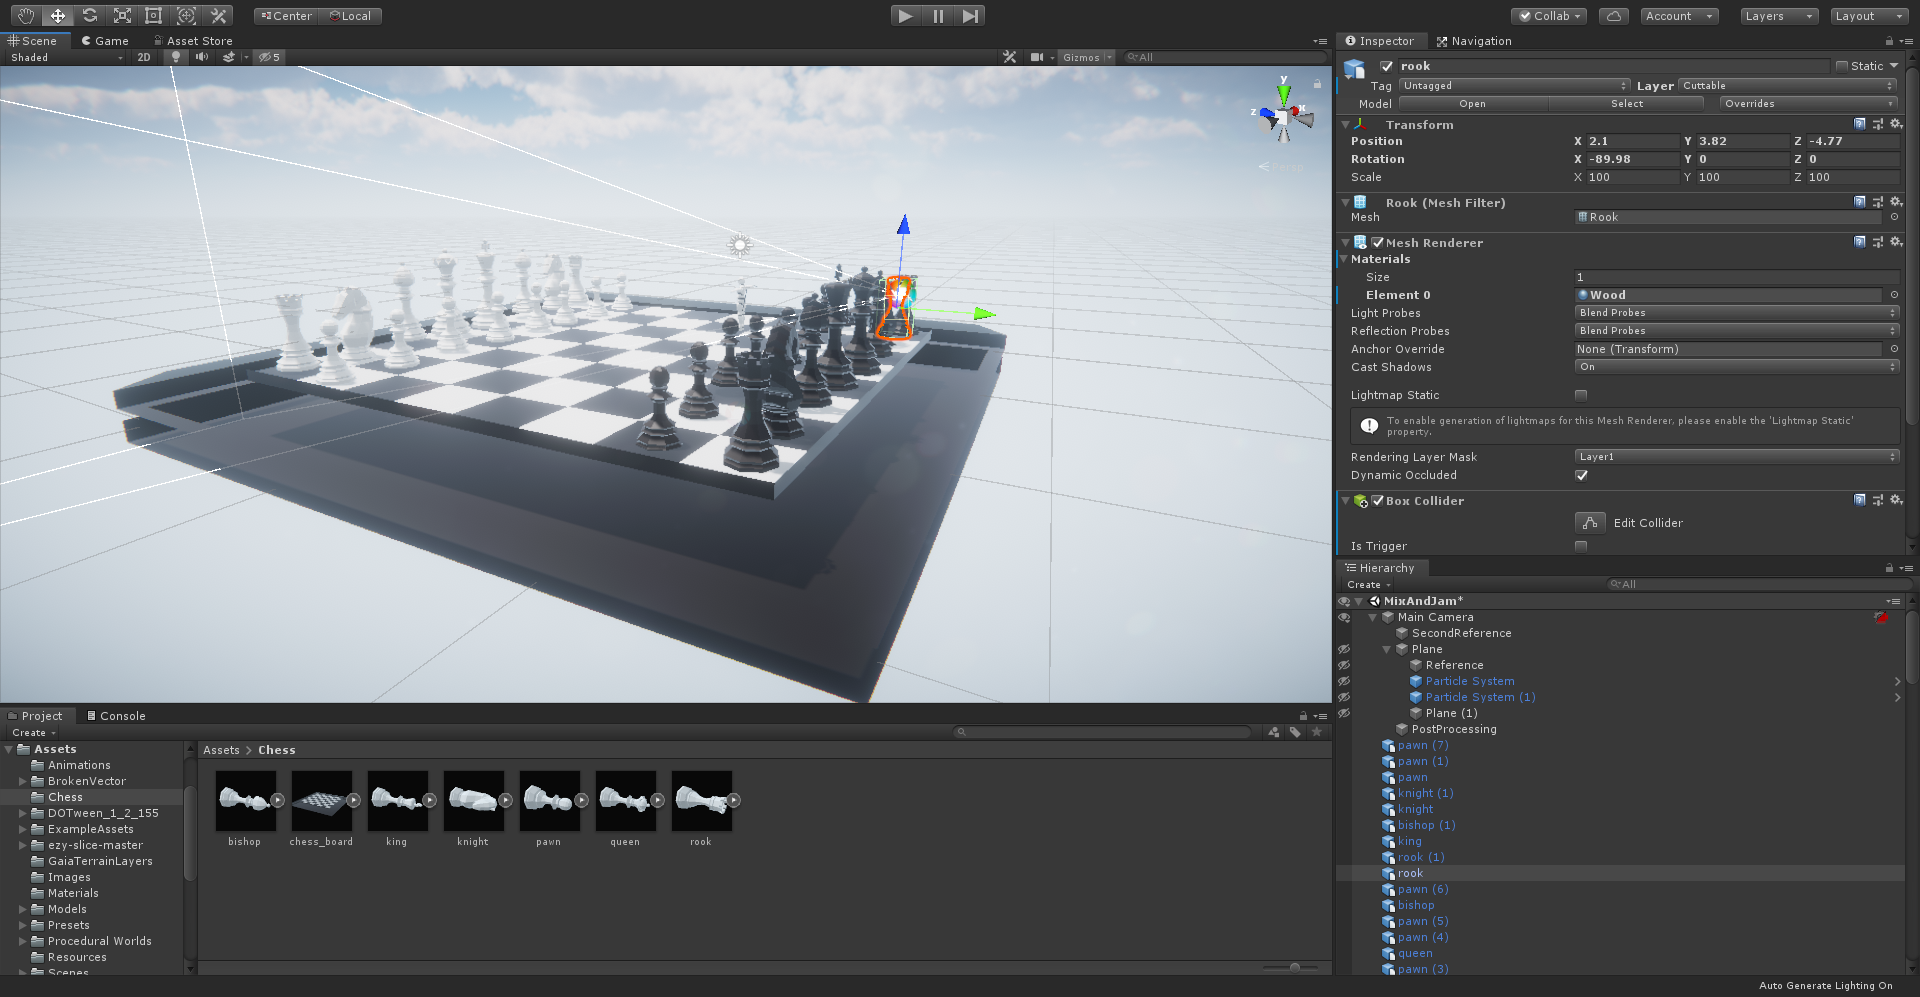
\includegraphics[width=\linewidth]{img/chess-scene.png}
    \captionsetup{justification=centering}
    \caption{La scacchiera vista dall'editor di Unity.} 
  \end{subfigure}
   \begin{subfigure}[b]{0.45\linewidth}
    \centering
    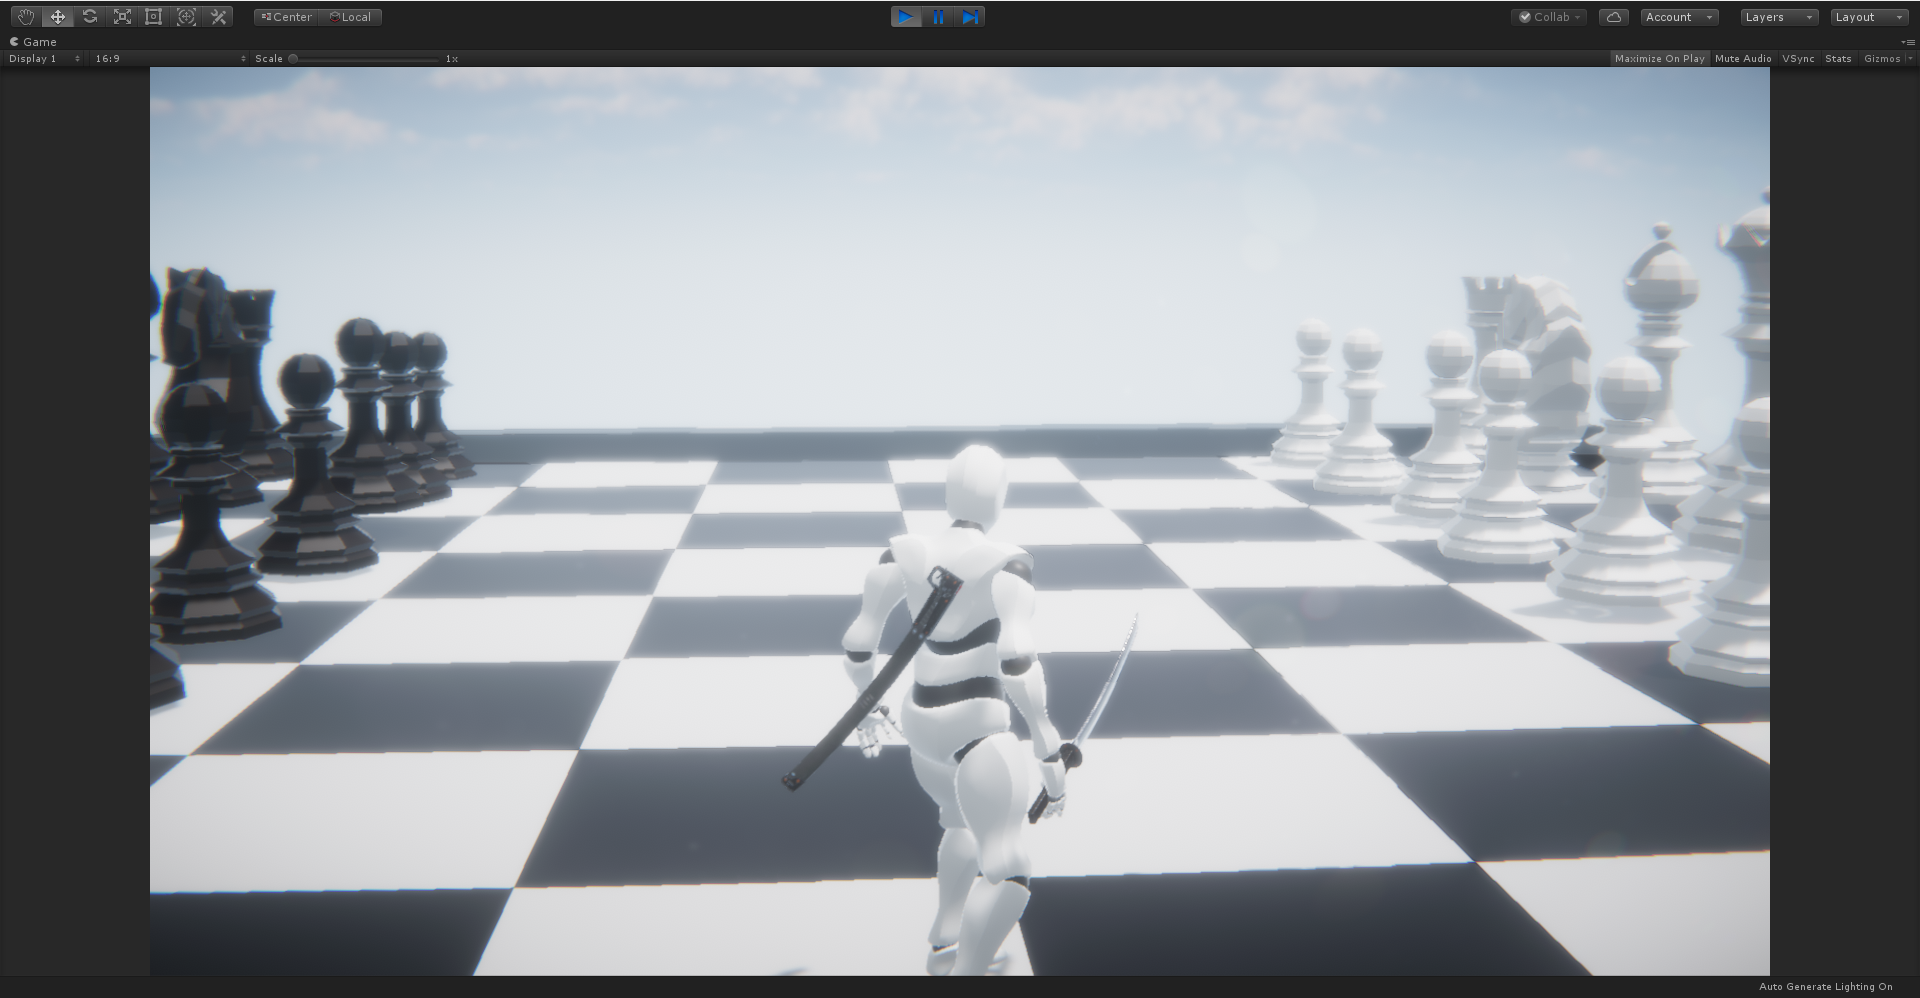
\includegraphics[width=\linewidth]{img/chess-in-game.png}
    \captionsetup{justification=centering}
    \caption{La schacchiera vista all'interno del gioco.}
  \end{subfigure}
\end{figure}

\subsubsection*{Gameplay}
Nel secondo livello è possibile interagire con gli oggetti ricreati (i pezzi degli scacchi) tagliandoli in vari pezzi la cui forma dipende dal movimento di taglio della spada del protagonista.

\begin{figure}[H]
  \centering
  \begin{subfigure}[b]{0.45\linewidth}
    \centering
    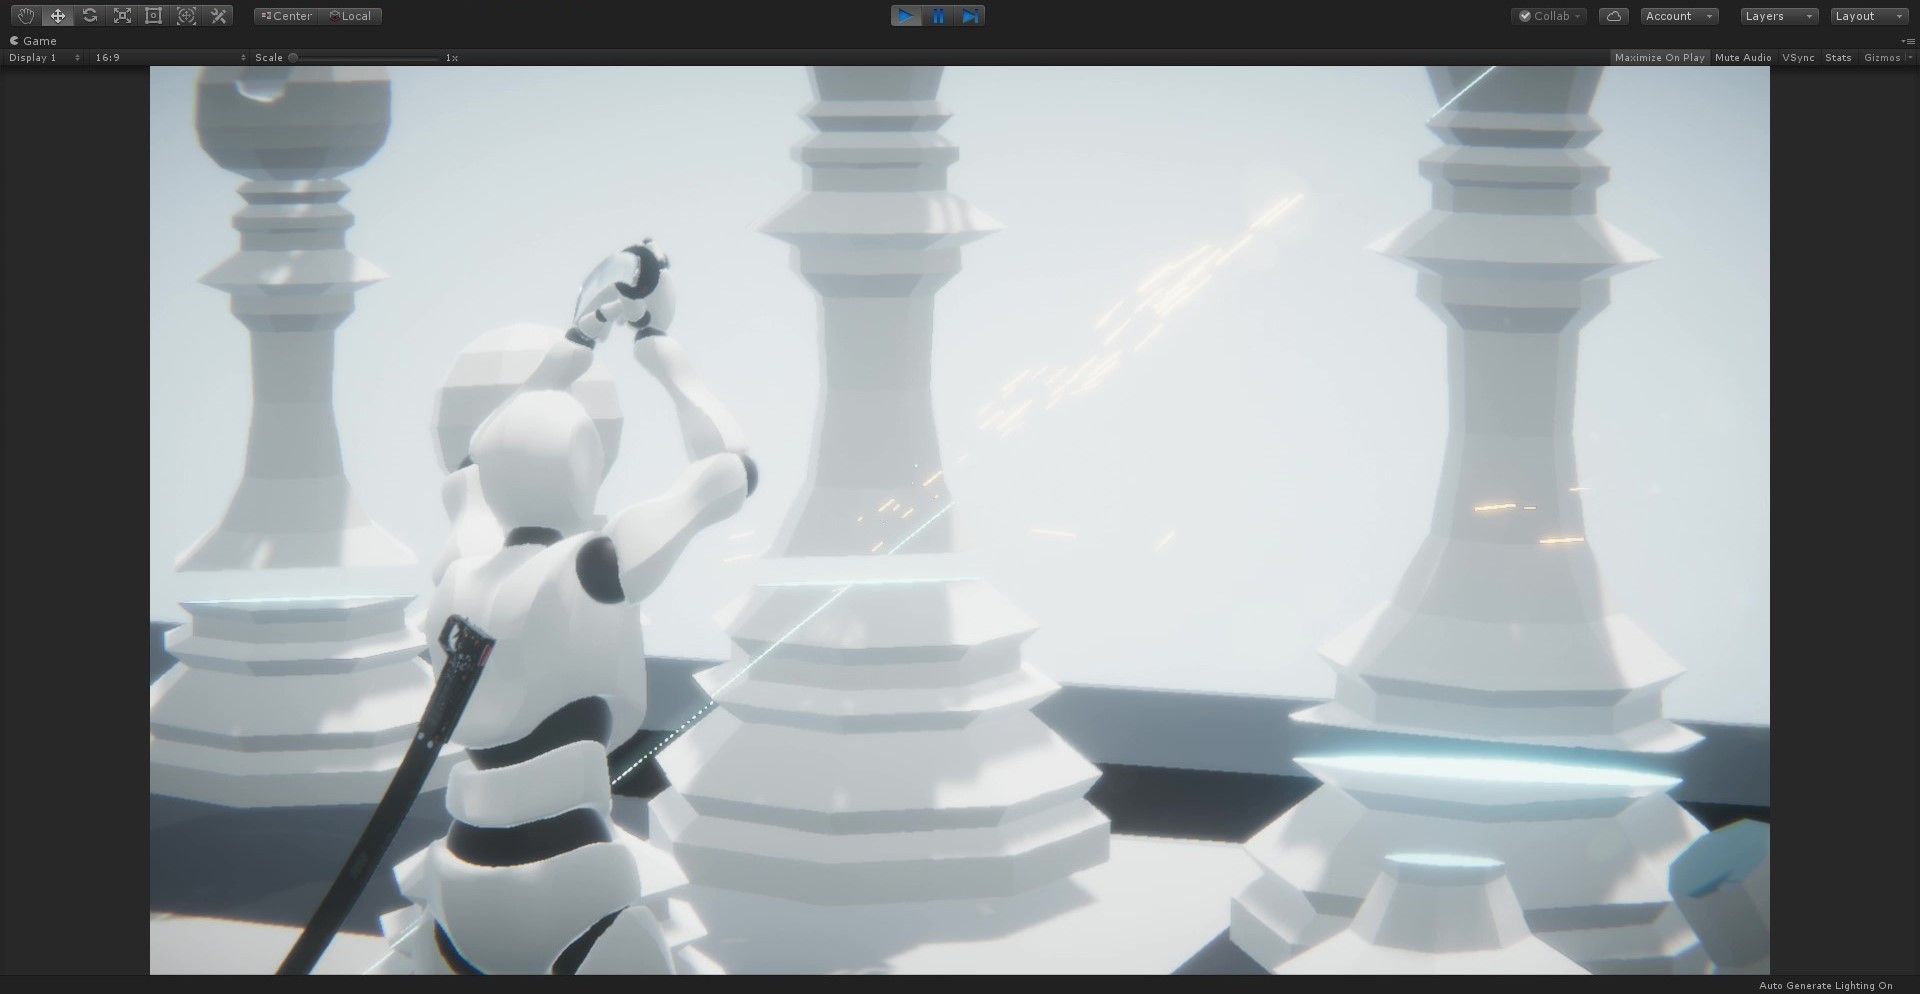
\includegraphics[width=\linewidth]{img/chess-game_Moment.jpg}
    \captionsetup{justification=centering}
    \caption{Il protagonista del gioco mentre taglia i pezzi}
  \end{subfigure}
   \begin{subfigure}[b]{0.45\linewidth}
    \centering
    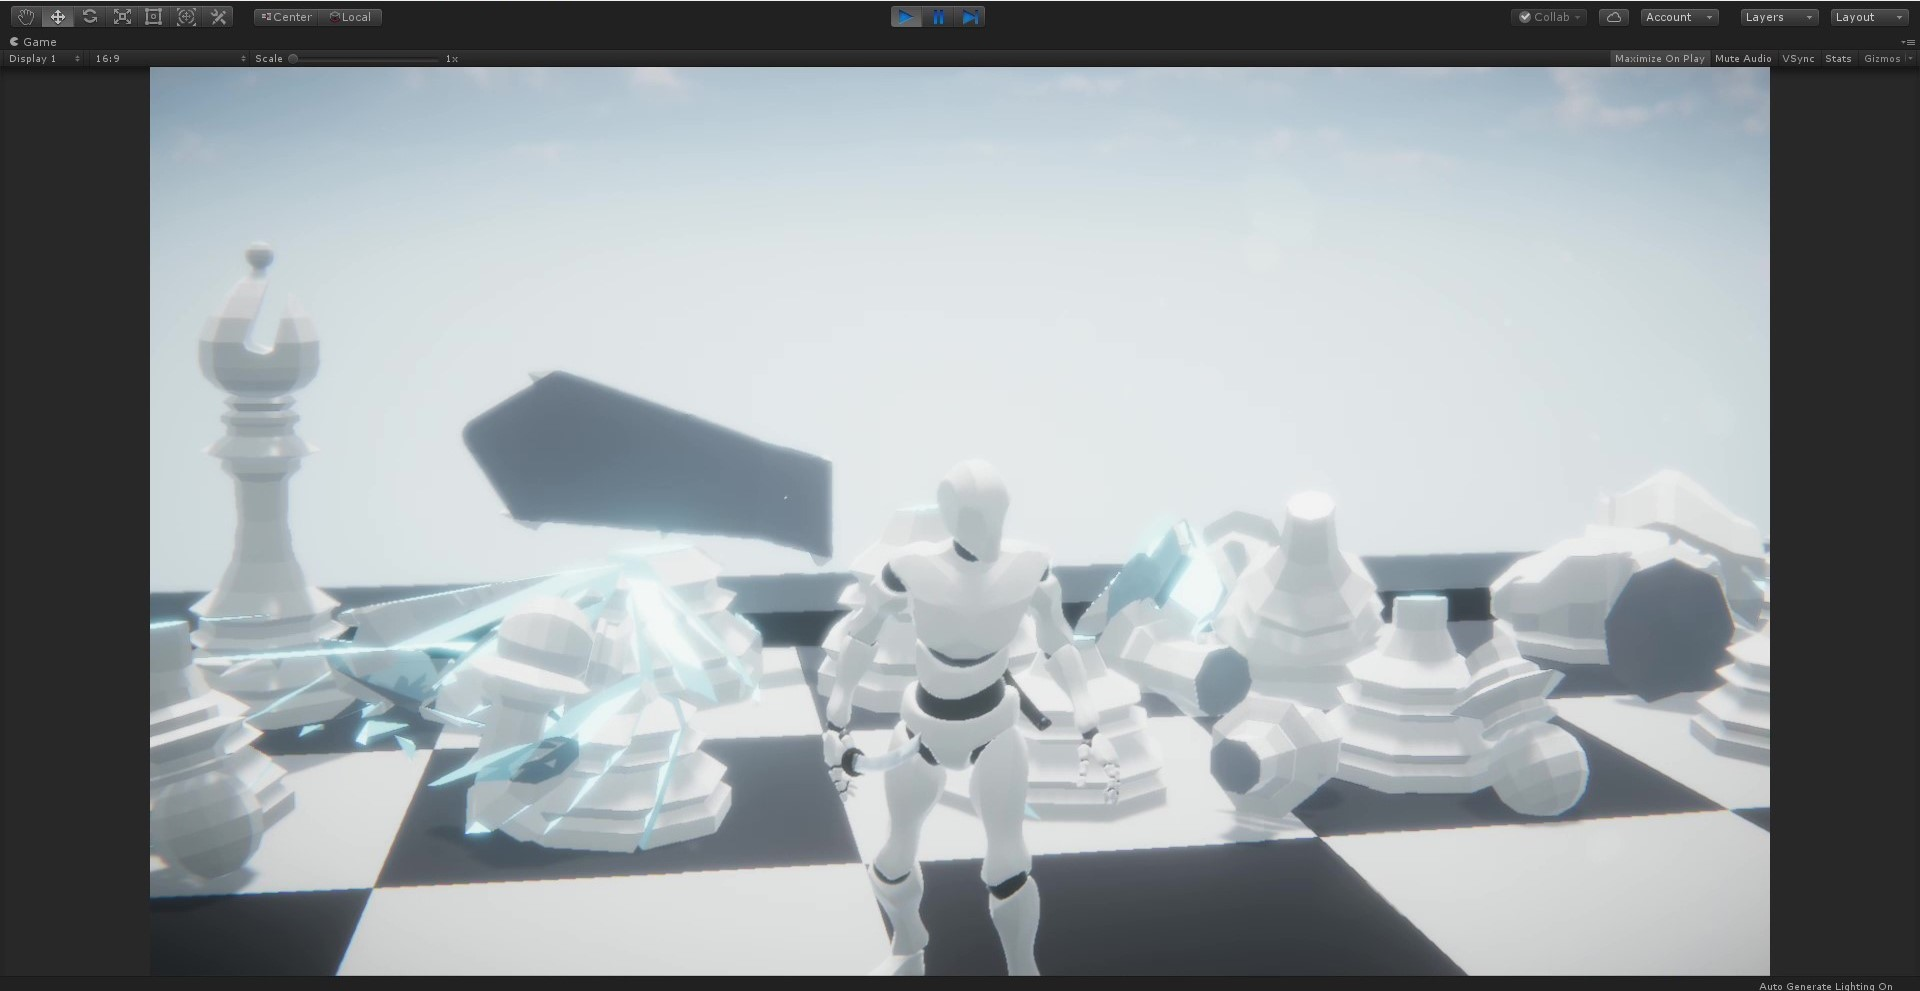
\includegraphics[width=\linewidth]{img/chess-game_cutted.jpg}
    \captionsetup{justification=centering}
    \caption{Il risultato dei precedenti tagli sui pezzi degli scacchi}
  \end{subfigure}
\end{figure}


\subsubsection*{Tecniche utilizzate}
\begin{itemize}
    \item Il gameplay risulta fluido poich\`e gli oggetti ricostruti hanno una geometria semplice e composta da un numero limitato di poligoni abbassando così il numero di calcoli da fare per effettuare il taglio.
    \item Per implementare il taglio degli oggetti abbiamo realizzato un piano parallelo al pavimento e l'abbiamo impostato come child della camera, in modo che si spostasse al movimento del giocatore.
    Per farlo ruotare sull'asse z lo abbiamo collegato all'asse x del movimento del mouse. Per effettivamente tagliare l'oggetto presente nel piano abbiamo utilizzato un framework open-source chiamato Ezy-Slice creato da DavidArayan (\url{https://github.com/DavidArayan/ezy-slice}).
    L'algoritmo utilizza delle coordinate baricentriche per generare dei nuovi set UV(ovvero le proiezioni di texture bidimensionale su un oggetto tridimensionale) per i triangoli. In sostanza l'algortimo utilizza dei "piani" per triangolare quali intersezioni tagliare individuate dai triangoli della mesh.
    
\end{itemize}

\chapter{Conclusioni}
Ringraziamo il Professor Marco Cristani per averci offerto questa opportunità in quanto è stato di nostro particolare gradimento lavorare su queste tematiche. Grazie a questa nostra esperienza abbiamo arricchito il nostro bagaglio di conoscenze, questo ci consentirà di affrontare al meglio gli studi a venire.

\section{Bibliografia}
\begin{itemize}
    \item Tutorial 3DF Zephyr su YouTube: \url{https://www.youtube.com/playlist?list=PLj8MbHn-bXVR5_e_h4LeG4Jzu1CM5atRH}
    \item Materiale del corso di Elaborazione di Segnali e Immagini del Professor Marco Cristani
    \item Photogrammetry Workflow di Unity: \url{https://unity3d.com/files/solutions/photogrammetry/Unity-Photogrammetry-Workflow_2017-07_v2.pdf}
    \item Documentazione ufficiale di Unity: \url{https://docs.unity3d.com/Manual/index.html}
    \item Wikipedia: \url{https://www.wikipedia.org/}
\end{itemize}



\end{document}
%END----------------------------------------------------
